\chapter{Dữ liệu và phương pháp nghiên cứu}
\label{ch:phuong-phap}

Chương này trình bày chi tiết kiến trúc hệ thống, quy trình xử lý dữ liệu và thiết kế các mô hình học máy trong khung thực nghiệm \textbf{DepSev-ML}. Để giải quyết các câu hỏi nghiên cứu đã đề ra, phương pháp luận được xây dựng dựa trên nguyên tắc module hóa, chuẩn tắc hóa quy trình tiền xử lý nhằm loại trừ rò rỉ dữ liệu, và thiết kế đa dạng các kiến trúc phân loại từ phẳng, phân cấp cứng/mềm đến thứ bậc.

\section{Tổng quan quy trình nghiên cứu DepSev-ML}
\label{sec:kien-truc-tong-the}

Khung làm việc DepSev-ML được tổ chức thành 7 cấu phần khoa học khép kín như mô tả trong Hình \ref{fig:overall-architecture}.

\begin{figure}[htbp]{Kiến trúc tổng thể 7 module của khung học máy thực nghiệm DepSev-ML}
\centering
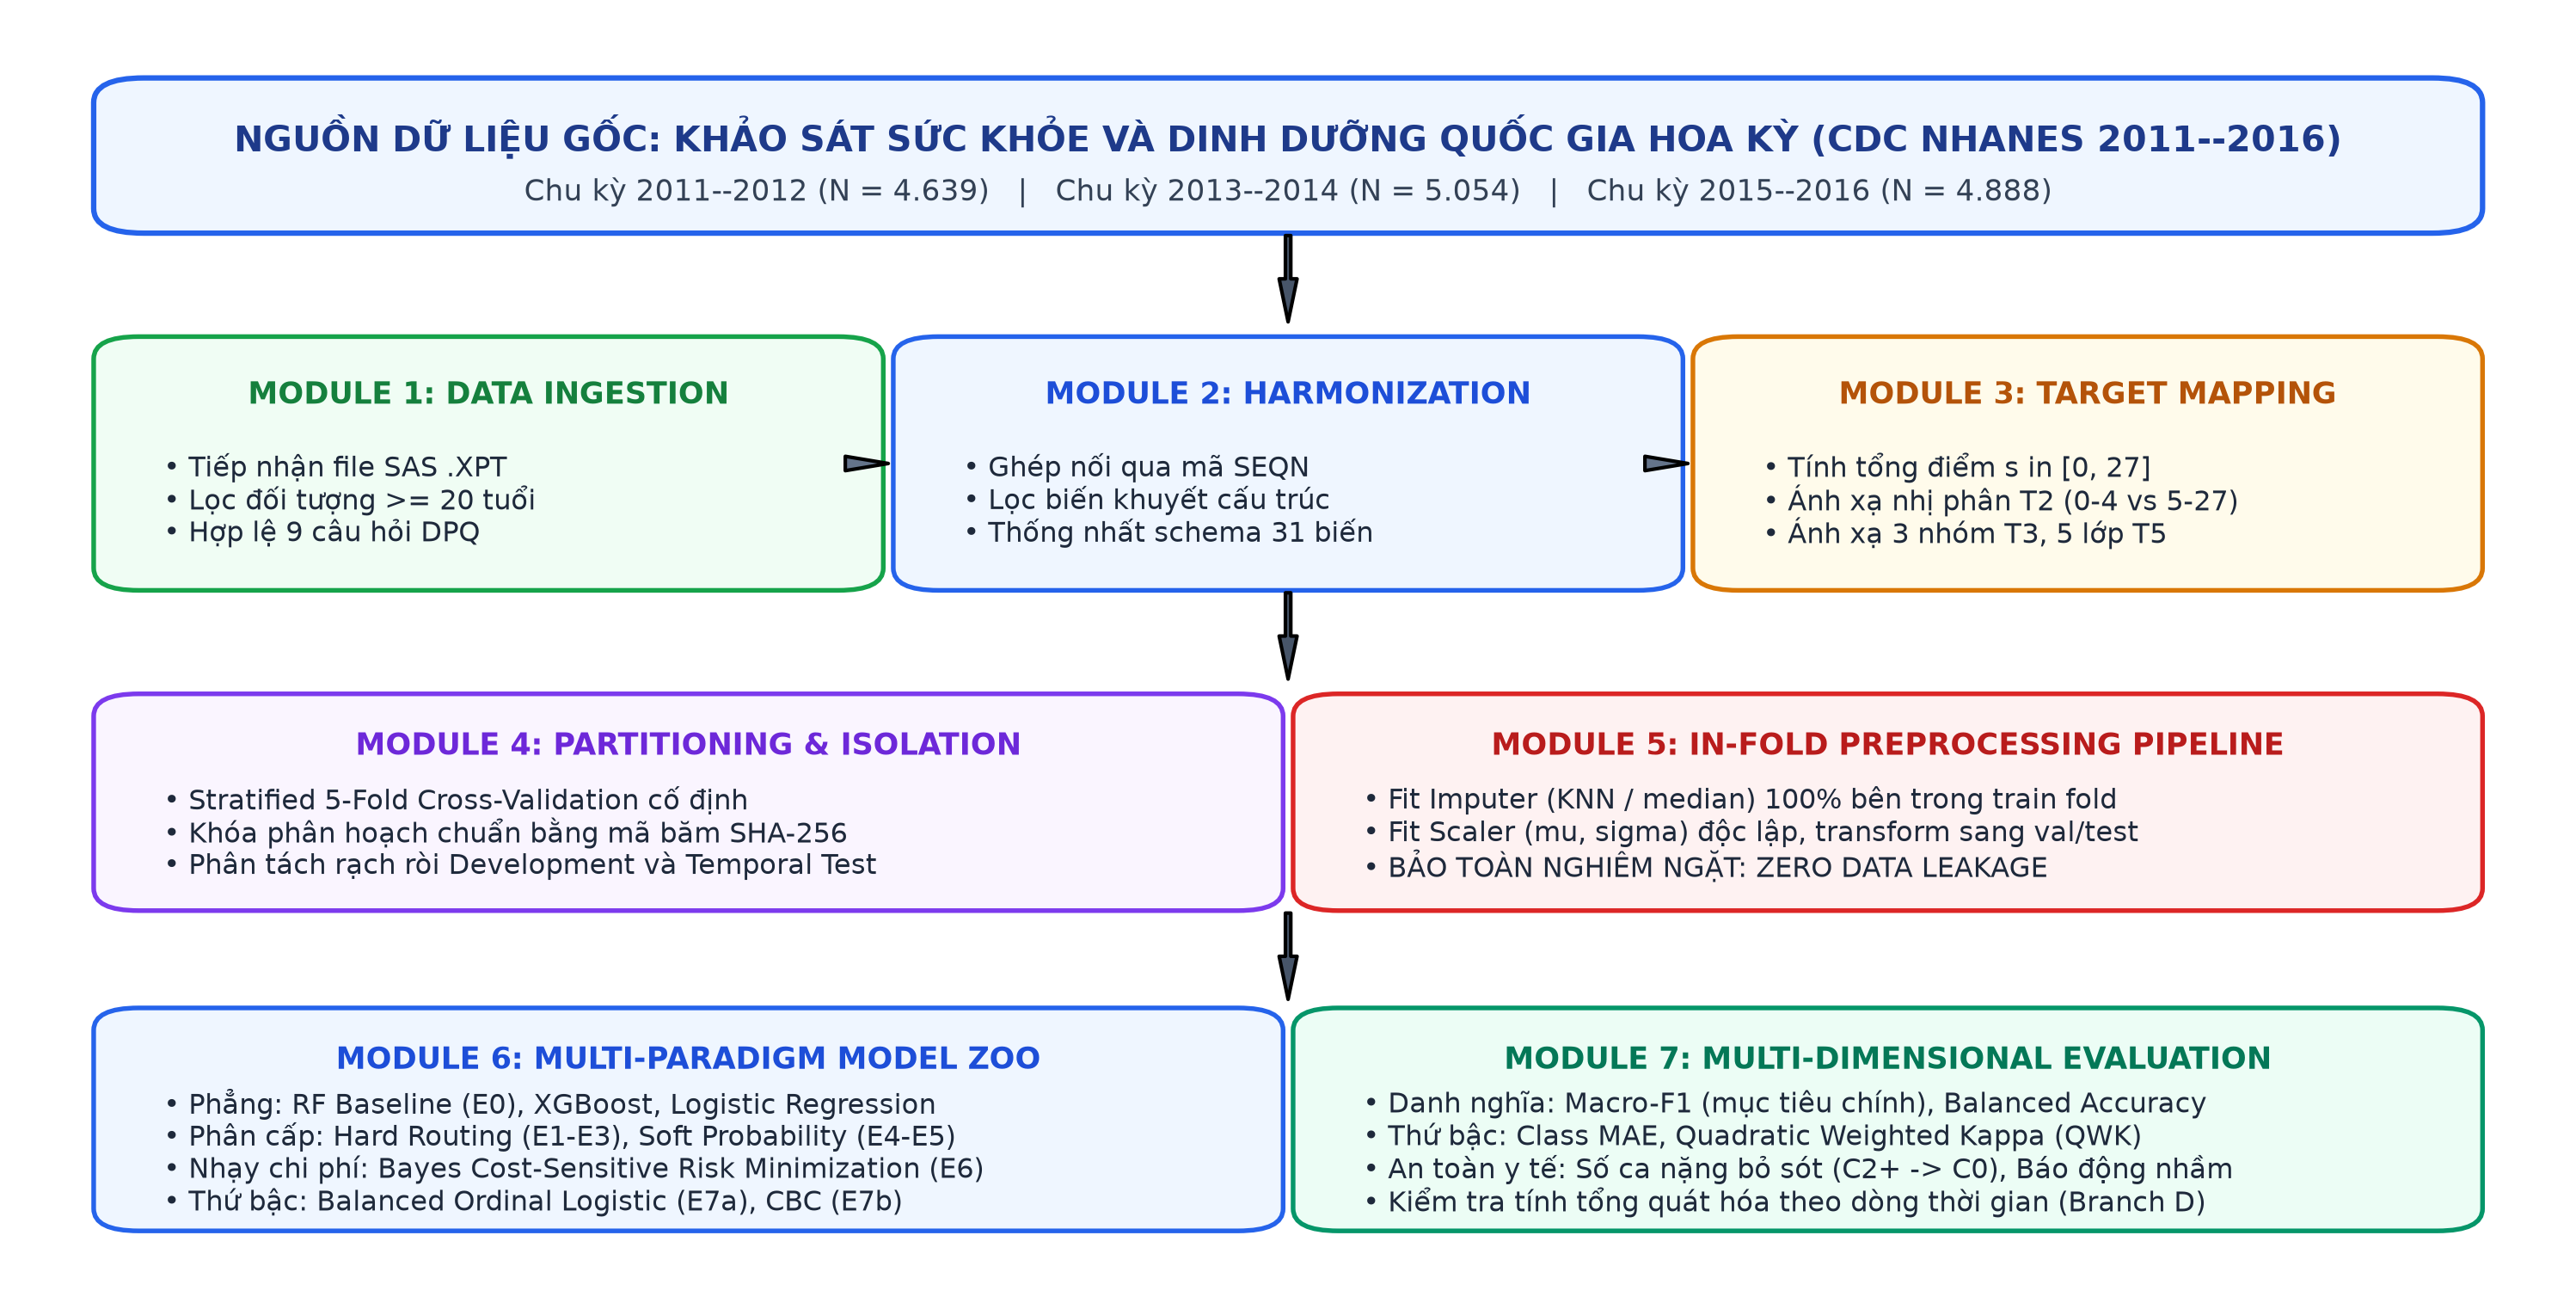
\includegraphics[width=\textwidth]{figures/depsev_overall_architecture.png}
\label{fig:overall-architecture}
\end{figure}
\FloatBarrier

Các cấu phần thực hiện các chức năng chuyên biệt:
\begin{enumerate}
    \item \textbf{Module 1 -- Data Ingestion \& Cohort Filtering:} Tiếp nhận các tệp dữ liệu gốc định dạng SAS Transport (.XPT) từ cổng thông tin CDC/NCHS, áp dụng bộ lọc tiêu chuẩn chọn đối tượng người trưởng thành ($\text{RIDAGEYR} \ge 20$) có đầy đủ 9 câu hỏi khảo sát DPQ hợp lệ.
    \item \textbf{Module 2 -- Harmonization \& Feature Engineering:} Ghép nối các bảng khảo sát và xét nghiệm qua mã định danh SEQN; chuẩn hóa tên biến, xử lý biến điều hướng phức tạp và loại bỏ các biến có tính khuyết thiếu cấu trúc giữa các chu kỳ.
    \item \textbf{Module 3 -- Target Space Mapping:} Ánh xạ tổng điểm PHQ-9 thành 4 không gian phân loại mục tiêu rời rạc ($T_2, T_3, T_4, T_5$) phục vụ khảo sát đa độ phân giải.
    \item \textbf{Module 4 -- Partitioning \& Isolation Engine:} Quản lý các phân hoạch dữ liệu cố định (Stratified 5-Fold CV Folds, Development/Held-out splits) bằng mã băm SHA-256 nhằm bảo đảm tính tái lập thực nghiệm tuyệt đối.
    \item \textbf{Module 5 -- Strict In-Fold Preprocessing Pipeline:} Thực thi quy trình điền khuyết (median/most-frequent), chuẩn hóa phương sai (StandardScaler) và mã hóa one-hot độc lập 100\% bên trong từng fold huấn luyện để triệt tiêu nguy cơ rò rỉ dữ liệu (Zero Data Leakage).
    \item \textbf{Module 6 -- Multi-Paradigm Model Zoo:} Triển khai và tích hợp 4 họ mô hình phân loại phẳng ($E_0$), 4 cấu hình phân cấp cứng ($E_1 \to E_3$), 4 cấu hình phân cấp mềm kết hợp tối ưu chi phí Bayes ($E_4 \to E_6$) và 4 cấu hình phân loại thứ bậc ($E_7$).
    \item \textbf{Module 7 -- Multi-Dimensional Evaluation Suite:} Đánh giá toàn diện trên cả hệ thống độ đo phân loại danh nghĩa (Macro-F1, Balanced Accuracy), độ đo hình học thứ bậc (Class MAE, Quadratic Weighted Kappa) và chỉ số an toàn lâm sàng.
\end{enumerate}

\section{Bộ dữ liệu NHANES và Quy trình tiền xử lý in-fold}
\label{sec:du-lieu-nghien-cuu}

\subsection{Tập dữ liệu phát triển Legacy (NHANES 2013--2014)}
\label{subsec:legacy-cohort}

Tập dữ liệu Legacy được xây dựng từ chu kỳ NHANES 2013--2014, gồm $N = 5.054$ đối tượng trưởng thành có dữ liệu PHQ-9 hợp lệ:
\begin{itemize}
    \item \textbf{Phân hoạch phát triển (Development Cohort):} Gồm $N = 4.045$ đối tượng, được sử dụng xuyên suốt cho các thực nghiệm Stratified 5-Fold CV, Feature Ablation, Nested Hyperparameter Tuning và chuỗi thực nghiệm chính $E_0 \to E_7$.
    \item \textbf{Phân hoạch kiểm tra bổ sung (Supplementary Held-out Cohort):} Gồm $N = 1.009$ đối tượng được lưu giữ riêng để tham khảo đối chứng. Cần ghi nhận tính chất lịch sử: 813 trong số 1.009 đối tượng này từng nằm trong tập phát triển ở các phiên bản tiền nghiệm, do đó tập này chỉ mang giá trị tham chiếu phụ trợ, toàn bộ kết luận khoa học cốt lõi dựa trên quy trình kiểm định chéo Stratified 5-Fold lồng nhau trên tập phát triển.
\end{itemize}

Phân bố chi tiết các mức độ triệu chứng PHQ-9 trên tập Legacy được tổng hợp trong Bảng \ref{tab:legacy-class-dist}. Tỷ lệ lớp thiểu số rất nặng $C_4$ chỉ chiếm 1.09\%, khẳng định tính chất mất cân bằng cực đoan của bài toán.

\begin{table}{Phân bố các lớp triệu chứng PHQ-9 trên tập dữ liệu Legacy ($N = 5.054$)}
\centering
\footnotesize
\setlength{\tabcolsep}{3pt}
\label{tab:legacy-class-dist}
\begin{tabularx}{\textwidth}{l c >{\centering\arraybackslash}X >{\centering\arraybackslash}X >{\centering\arraybackslash}X >{\centering\arraybackslash}X >{\centering\arraybackslash}X}
\toprule
\textbf{Phân hoạch} & \textbf{Tổng $N$} & \textbf{$C_0$ (0--4)} & \textbf{$C_1$ (5--9)} & \textbf{$C_2$ (10--14)} & \textbf{$C_3$ (15--19)} & \textbf{$C_4$ (20--27)} \\
\midrule
Development & 4.045 & 3.016 (74.56\%) & 638 (15.77\%) & 243 (6.01\%) & 104 (2.57\%) & 44 (1.09\%) \\
Held-out & 1.009 & 748 (74.13\%) & 162 (16.06\%) & 60 (5.95\%) & 28 (2.78\%) & 11 (1.09\%) \\
\midrule
\textbf{Toàn bộ} & \textbf{5.054} & \textbf{3.764 (74.48\%)} & \textbf{800 (15.83\%)} & \textbf{303 (6.00\%)} & \textbf{132 (2.61\%)} & \textbf{55 (1.09\%)} \\
\bottomrule
\end{tabularx}
\end{table}

\subsection{Tập dữ liệu đa chu kỳ chính thức (Official Multi-Cycle Cohort)}
\label{subsec:multicycle-cohort}

Để kiểm tra tính ổn định trên quy mô lớn và đánh giá khả năng tổng quát hóa theo dòng thời gian, nghiên cứu tiến hành trích xuất và hài hòa hóa dữ liệu từ ba chu kỳ NHANES liên tiếp: 2011--2012, 2013--2014 và 2015--2016, nâng tổng quy mô lên $N = 14.581$ đối tượng (Bảng \ref{tab:multicycle-class-dist}).

\begin{table}{Quy mô và phân bố các lớp triệu chứng trên các chu kỳ NHANES chính thức}
\centering
\footnotesize
\setlength{\tabcolsep}{3pt}
\label{tab:multicycle-class-dist}
\begin{tabularx}{\textwidth}{l c >{\centering\arraybackslash}X >{\centering\arraybackslash}X >{\centering\arraybackslash}X >{\centering\arraybackslash}X >{\centering\arraybackslash}X}
\toprule
\textbf{Chu kỳ / Phân nhánh} & \textbf{Tổng $N$} & \textbf{$C_0$ (\%)} & \textbf{$C_1$ (\%)} & \textbf{$C_2$ (\%)} & \textbf{$C_3$ (\%)} & \textbf{$C_4$ (\%)} \\
\midrule
NHANES 2011--2012 & 4.639 & 76.12\% & 14.79\% & 5.22\% & 2.61\% & 1.27\% \\
NHANES 2013--2014 (Branch A) & 5.054 & 74.48\% & 15.83\% & 6.00\% & 2.61\% & 1.09\% \\
NHANES 2015--2016 (Branch D Test) & 4.888 & 74.65\% & 17.21\% & 5.03\% & 2.03\% & 1.08\% \\
\midrule
\textbf{Pooled 2011--2016 (Branch B)} & \textbf{14.581} & \textbf{75.06\%} & \textbf{15.96\%} & \textbf{5.42\%} & \textbf{2.41\%} & \textbf{1.15\%} \\
\bottomrule
\end{tabularx}
\end{table}

\subsection{Quy trình tiền xử lý và nguyên tắc Zero Data Leakage}
\label{subsec:data-pipeline}

Quy trình tiền xử lý và hài hòa hóa dữ liệu được chuẩn hóa thành một đường ống xử lý tự động như trình bày trong Hình \ref{fig:data-pipeline}.

\begin{figure}[htbp]{Quy trình tiền xử lý dữ liệu in-fold và nguyên tắc cách ly bảo toàn Zero Data Leakage}
\centering
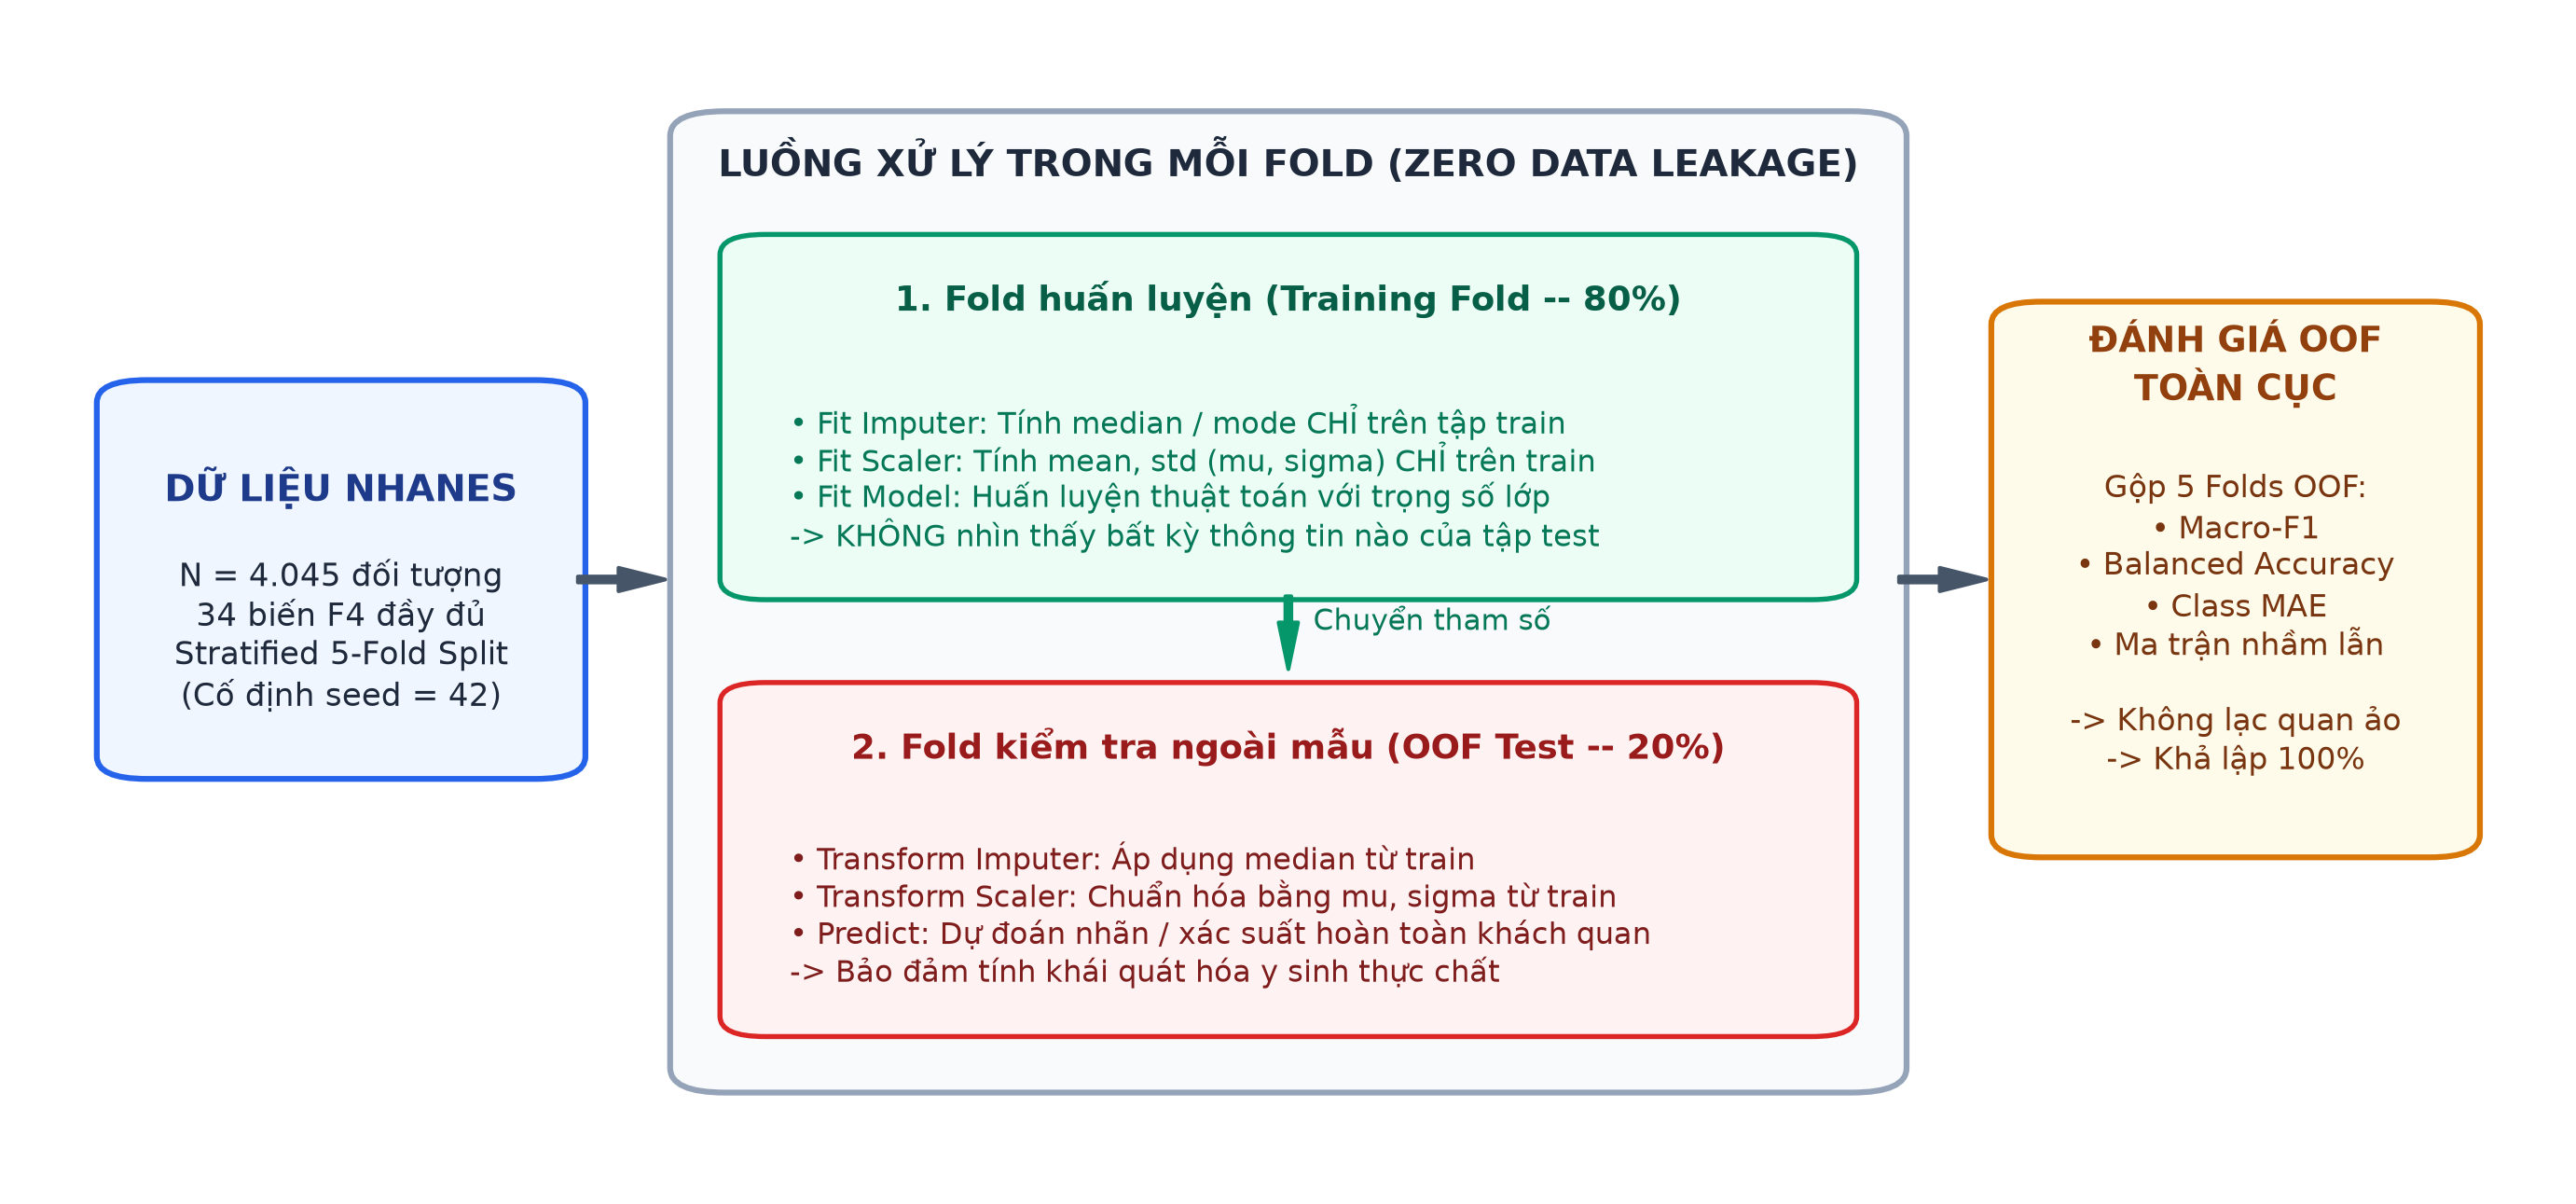
\includegraphics[width=\textwidth]{figures/fig3_infold_cv_pipeline.png}
\label{fig:data-pipeline}
\end{figure}
\FloatBarrier

Quy trình bảo đảm nguyên tắc nghiêm ngặt:
\begin{enumerate}
    \item \textbf{Loại trừ biến khuyết cấu trúc:} Biến số xét nghiệm Triglyceride chỉ được lấy mẫu trên nhóm đối tượng nhịn ăn sáng ở một số chu kỳ, dẫn đến tỷ lệ khuyết thiếu cấu trúc vượt quá 50\%; biến này bị loại bỏ hoàn toàn để bảo đảm tính đồng nhất của 31 đặc trưng lõi ($F_{4\_\text{common31}}$).
    \item \textbf{Cô lập tham số in-fold:} Các phép tính thống kê phục vụ điền khuyết (giá trị trung vị của biến liên tục, giá trị xuất hiện nhiều nhất của biến phân loại) và các tham số chuẩn hóa phương sai ($\mu, \sigma$ của \texttt{StandardScaler}) được tính toán độc lập 100\% trên tập huấn luyện của fold hiện tại, sau đó mới dùng các tham số này để biến đổi tập kiểm tra.
    \item \textbf{Bảo toàn hoàn toàn nhãn mục tiêu:} Tuyệt đối không đưa bất kỳ câu hỏi nào trong 9 mục khảo sát DPQ vào ma trận đặc trưng đầu vào $\mathbf{X}$.
\end{enumerate}

\section{Xây dựng không gian đặc trưng lũy tiến ($F_1 \to F_4$)}
\label{sec:he-thong-dac-trung}

Để khảo sát thực nghiệm đóng góp của từng miền thông tin y sinh học (RQ1), DepSev-ML tổ chức 34 biến số đầu vào thành 4 nhóm đặc trưng lũy tiến ($F_1 \to F_4$) như mô tả trong Hình \ref{fig:feature-groups}.

\begin{figure}[htbp]{Cấu trúc 4 không gian đặc trưng lũy tiến $F_1 \to F_4$ trong DepSev-ML}
\centering
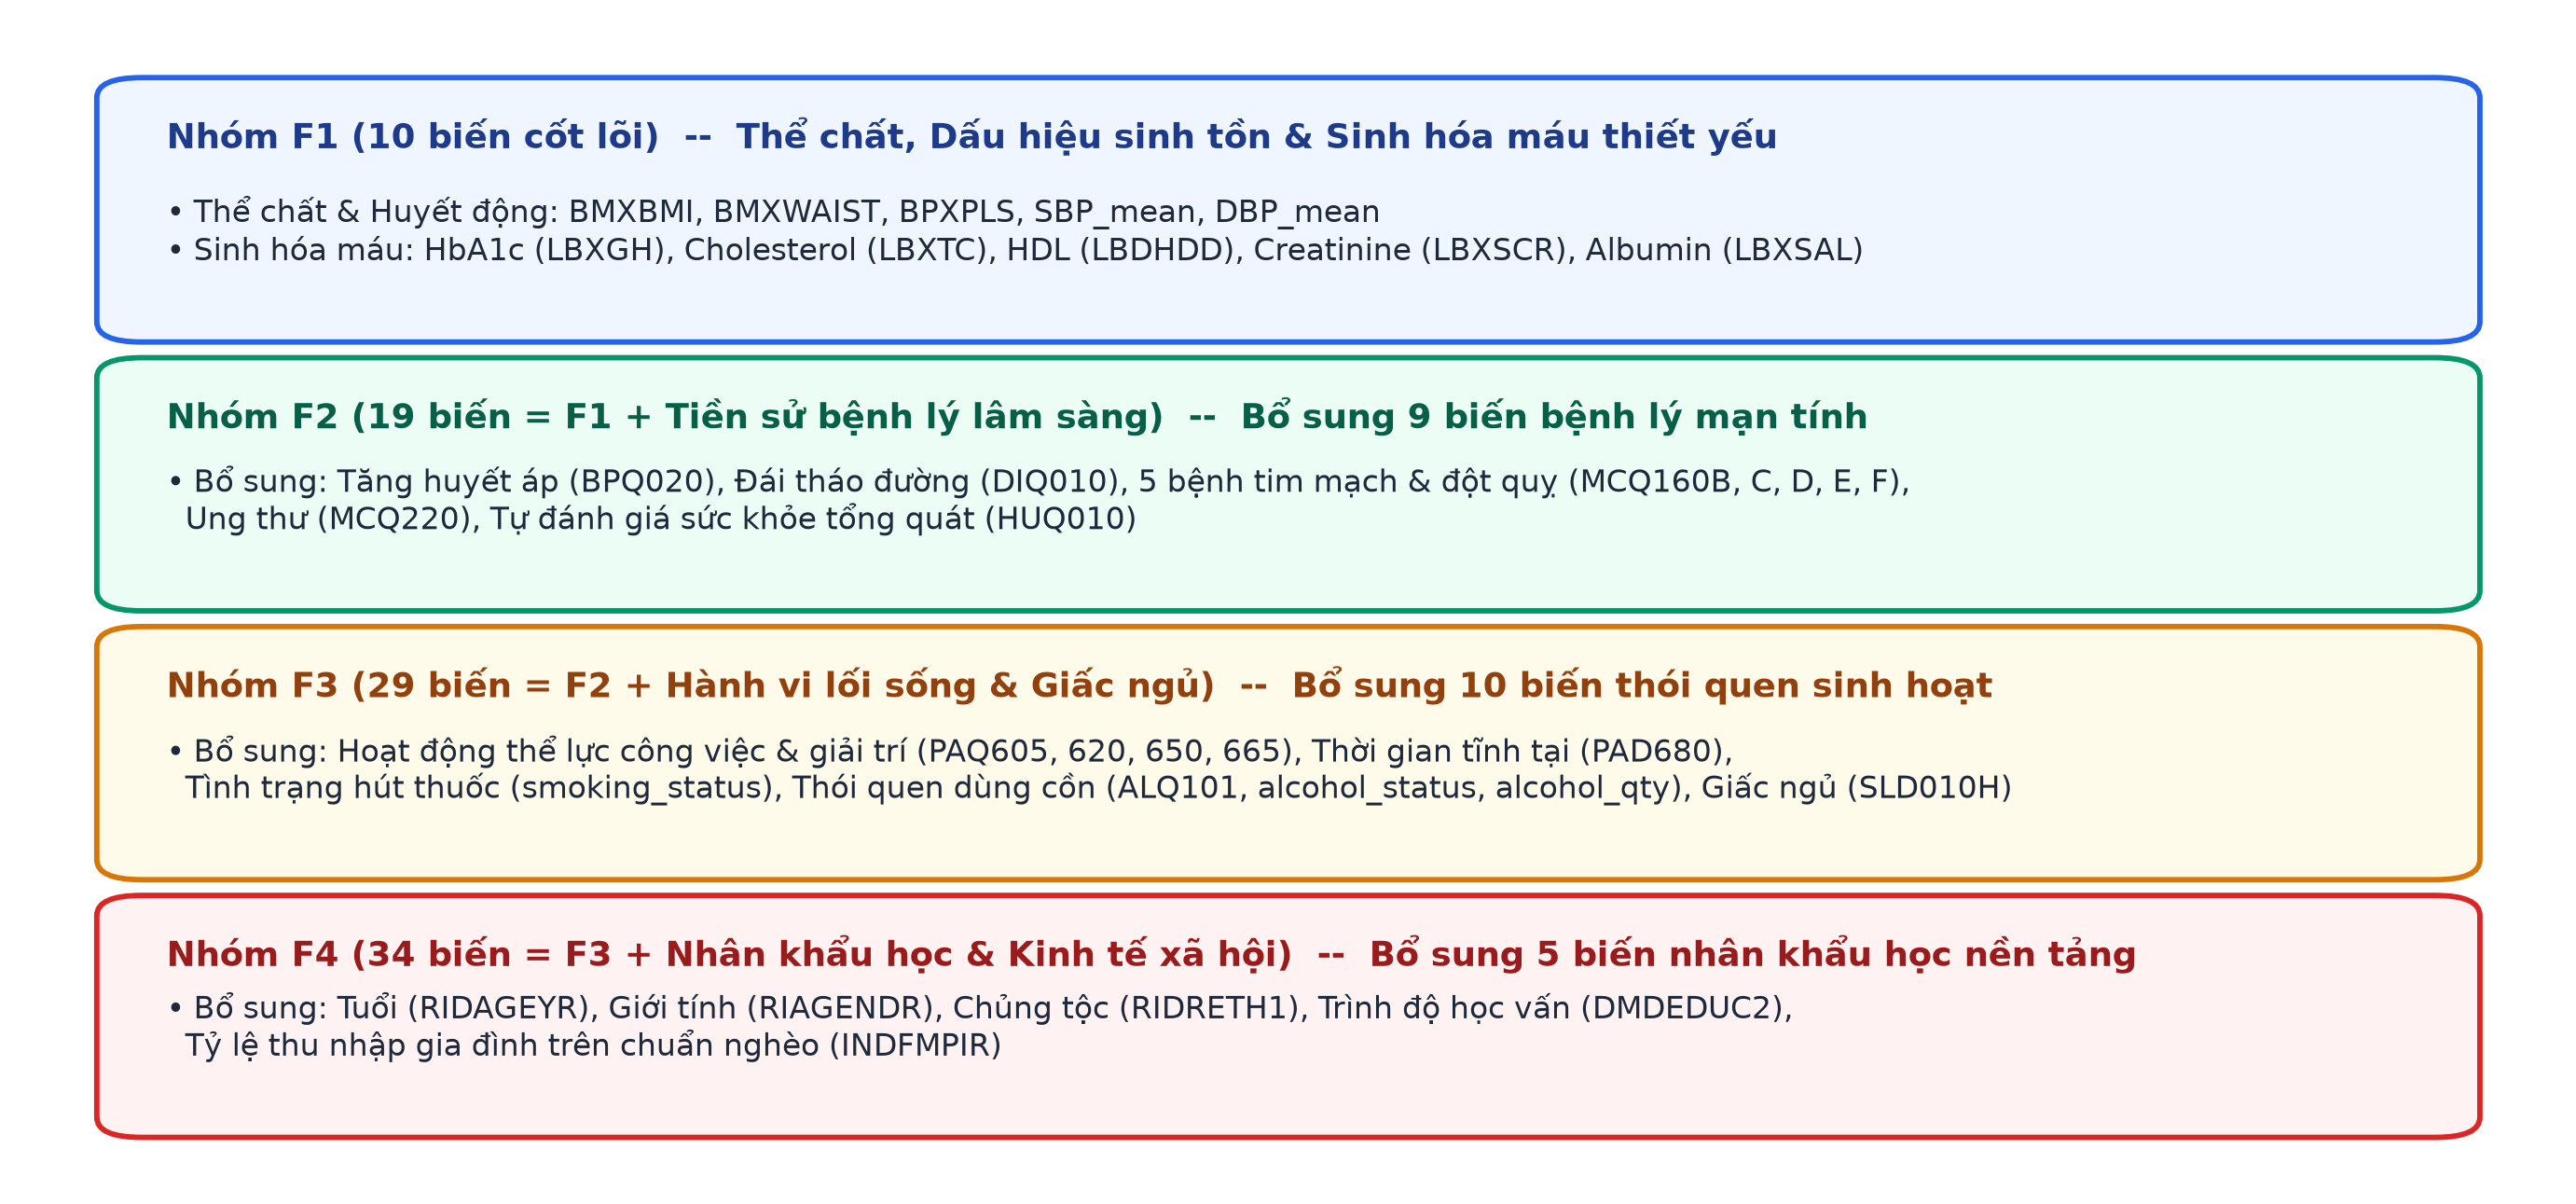
\includegraphics[width=\textwidth]{figures/fig3_3_feature_groups.png}
\label{fig:feature-groups}
\end{figure}
\FloatBarrier

Các không gian đặc trưng được xác lập chính thức gồm:
\begin{itemize}
    \item \textbf{Không gian $F_1$ (10 biến cốt lõi):} Gồm 5 chỉ số nhân trắc học và huyết động (BMI, chu vi vòng eo, nhịp tim nghỉ, huyết áp tâm thu trung bình, huyết áp tâm trương trung bình) kết hợp cùng 5 chỉ số xét nghiệm sinh hóa máu thiết yếu (HbA1c, Cholesterol toàn phần, HDL, Creatinine và Albumin).
    \item \textbf{Không gian $F_2$ (19 biến = $F_1$ + Tiền sử bệnh lâm sàng):} Bổ sung 9 biến bệnh lý mạn tính: tăng huyết áp, đái tháo đường, 5 bệnh lý tim mạch và đột quỵ, tiền sử ung thư và tự đánh giá sức khỏe tổng quát.
    \item \textbf{Không gian $F_3$ (29 biến = $F_2$ + Lối sống \& Giấc ngủ):} Bổ sung 10 chỉ số hành vi: hoạt động thể lực tại nơi làm việc và giải trí, thời gian tĩnh tại mỗi ngày, tình trạng hút thuốc, thói quen sử dụng rượu bia và thời lượng giấc ngủ ban đêm.
    \item \textbf{Không gian $F_4$ (34 biến = $F_3$ + Nhân khẩu học \& Kinh tế xã hội):} Bổ sung 5 biến nhân khẩu học nền tảng: tuổi, giới tính sinh học, chủng tộc, trình độ học vấn và tỷ lệ thu nhập gia đình trên chuẩn nghèo (INDFMPIR).
\end{itemize}

Bảng \ref{tab:feature-summary} tóm tắt cấu trúc phân nhóm đặc trưng; danh mục chi tiết 34 biến kèm mã định danh CDC được trình bày đầy đủ tại Phụ lục \ref{app:feature-inventory}.

\begin{table}{Tóm tắt cấu trúc 4 không gian đặc trưng lũy tiến trong DepSev-ML}
\centering
\footnotesize
\setlength{\tabcolsep}{4pt}
\label{tab:feature-summary}
\begin{tabularx}{\textwidth}{l c p{5.5cm} X}
\toprule
\textbf{Không gian} & \textbf{Số biến} & \textbf{Các nhóm biến thành phần} & \textbf{Ý nghĩa lâm sàng và dịch tễ học} \\
\midrule
$F_1$ & 10 & Thể chất, Sinh tồn \& Xét nghiệm máu thiết yếu & Phản ánh chuyển hóa cơ bản, huyết động và viêm mạn tính \\
$F_2$ & 19 & $F_1$ + 9 tiền sử bệnh lý mạn tính & Tích hợp chẩn đoán tiền sử của bác sĩ và tự đánh giá sức khỏe \\
$F_3$ & 29 & $F_2$ + 10 hành vi lối sống \& giấc ngủ & Bổ sung nhịp sinh học, mức độ vận động và hành vi kích thích \\
$F_4$ & 34 & $F_3$ + 5 nhân khẩu học \& kinh tế xã hội & Bổ sung yếu tố nguy cơ xã hội, độ tuổi và áp lực kinh tế \\
\midrule
$F_{4\_\text{common31}}$ & 31 & 31 biến đồng nhất trên cả 3 chu kỳ NHANES & Chuẩn hóa schema phục vụ kiểm định đa chu kỳ Pooled \\
\bottomrule
\end{tabularx}
\end{table}

\section{Xây dựng nhãn PHQ-9 và các không gian mục tiêu ($T_2 \to T_5$)}
\label{sec:nhan-muc-tieu}

Từ tổng điểm PHQ-9 liên tục $s \in [0, 27]$, nghiên cứu thiết lập 4 không gian phân loại mục tiêu:
\begin{itemize}
    \item $T_2$ ($K=2$): Nhị phân giữa $C_0$ ($s \in [0, 4]$) và nhóm có triệu chứng ($s \in [5, 27]$).
    \item $T_3$ ($K=3$): Ba nhóm gộp quy ước gồm $C_0$ ($0$--$4$, 74.6\%), $C_1$ ($5$--$9$, 15.8\%) và $C_2^+$ ($10$--$27$, 9.7\%). Nhóm $C_2^+$ được quy ước là "nhóm Nặng quy ước" (Severe convention) bao gồm toàn bộ các ca từ Moderate đến Severe chuẩn.
    \item $T_4$ ($K=4$): Bốn mức gồm $C_0$ ($0$--$4$), $C_1$ ($5$--$9$), $C_2$ ($10$--$14$), và $C_3^+$ ($15$--$27$).
    \item $T_5$ ($K=5$): Năm mức độ lâm sàng chuẩn PHQ-9 gồm $C_0$ (Minimal), $C_1$ (Mild), $C_2$ (Moderate), $C_3$ (Moderately severe), và $C_4$ (Severe).
\end{itemize}

\section{Quy trình áp dụng Random Forest trên dữ liệu thực tế NHANES}
\label{sec:xay-dung-random-forest}

Rừng ngẫu nhiên (Random Forest) đóng vai trò là mô hình học máy xương sống (Backbone Baseline) trong toàn bộ khung nghiên cứu DepSev-ML. Để bảo đảm tính minh bạch và chuẩn tắc cao nhất, quy trình phát triển, huấn luyện và kiểm định mô hình Random Forest trên dữ liệu thực tế NHANES được chuẩn hóa qua các bước thực nghiệm liên hoàn:

\begin{enumerate}
    \item \textbf{Bước 1 -- Xác lập tập dữ liệu và không gian đặc trưng:} 
    Mô hình được áp dụng trên tập dữ liệu phát triển Legacy gồm $N = 4.045$ đối tượng với không gian 34 đặc trưng đầy đủ ($F_4$). Phân phối nhãn 5 lớp mang tính mất cân bằng cực đoan: $C_0$ chiếm $3.016$ ca (74.56\%), $C_1$ chiếm $638$ ca (15.77\%), $C_2$ chiếm $243$ ca (6.01\%), $C_3$ chiếm $104$ ca (2.57\%) và $C_4$ chỉ có $44$ ca (1.09\%), tạo tỷ số mất cân bằng lên tới $68.5:1$.
    
    \item \textbf{Bước 2 -- Thiết lập phân hoạch Stratified 5-Fold Cross-Validation:} 
    Dữ liệu được phân chia thành 5 folds bằng cơ chế Stratified cố định hạt giống ngẫu nhiên \texttt{random\_state = 42}, bảo đảm tỷ lệ giữa 5 lớp nhãn luôn đồng nhất giữa tập huấn luyện (4 folds, $\approx 3.236$ mẫu) và tập kiểm định (1 fold, $\approx 809$ mẫu). Cấu trúc kiểm định lồng nhau (Nested CV: Outer 5 folds, Inner 3 folds) được thiết lập để tìm kiếm siêu tham số mà không tiếp xúc với tập kiểm tra của fold ngoài.
    
    \item \textbf{Bước 3 -- Thực thi tiền xử lý in-fold bảo toàn Zero Data Leakage:} 
    Để triệt tiêu hoàn toàn nguy cơ rò rỉ dữ liệu (Zero Data Leakage, Hình \ref{fig:data-pipeline}), quy trình điền khuyết giá trị thiếu (median cho biến liên tục, mode cho biến phân loại) và chuẩn hóa phân phối (\texttt{StandardScaler}) được tính toán độc lập bên trong từng fold huấn luyện, sau đó mới dùng các tham số đã học để biến đổi fold kiểm định.
    
    \item \textbf{Bước 4 -- Cấu hình siêu tham số chuẩn tắc (Frozen RF Spec):} 
    Bộ tham số tối ưu thu được từ Nested CV được chuẩn hóa và cố định chính thức thành cấu hình chuẩn: \texttt{n\_estimators = 150}, \texttt{max\_depth = 8}, \texttt{max\_features = 0.5}, \texttt{min\_samples\_split = 10}, \texttt{min\_samples\_leaf = 8}, \texttt{criterion = 'gini'}, \texttt{random\_state = 42}. Đặc biệt, kỹ thuật \texttt{class\_weight = 'balanced\_subsample'} được kích hoạt, tự động điều chỉnh trọng số nghịch đảo tần số lớp trên từng mẫu bootstrap riêng biệt của mỗi cây, gia tăng trọng số phạt cho các ca trầm cảm nặng.
    
    \item \textbf{Bước 5 -- Huấn luyện và tổng hợp suy luận Soft Voting:} 
    Quần thể $150$ cây quyết định con được huấn luyện độc lập trên các tập con bootstrap. Khi suy luận trên fold kiểm định, mẫu dữ liệu được truyền qua toàn bộ $150$ cây và xuất ra phân phối xác suất trung bình liên tục (Soft Voting) theo công thức $\bar{P}(Y = k \mid \mathbf{x}) = \frac{1}{150}\sum_{b=1}^{150} P_b(Y = k \mid \mathbf{x})$.
    
    \item \textbf{Bước 6 -- Đánh giá hiệu năng và chuẩn bị chuyển giao nghiên cứu:} 
    Mô hình được đánh giá thông qua hệ thống độ đo đa chiều: Macro-F1 (đo độ nhận diện cân bằng lớp hiếm), Balanced Accuracy, Weighted-F1, Brier Score và Class MAE. Toàn bộ kết quả thực nghiệm chi tiết của RF trên bài toán 5 lớp $T_5$, phân tích ma trận nhầm lẫn và sự suy thoái của lớp trung gian $C_1$ sẽ được trình bày tại Chương \ref{ch:thuc-nghiem}. Những hạn chế cốt lõi quan sát được trên $T_5$ chính là động lực khoa học trực tiếp dẫn đến việc tái cấu trúc sang bài toán phân cấp hai giai đoạn $T_3$.
\end{enumerate}

\section{Thiết kế các kiến trúc phân loại phân cấp hai giai đoạn ($T_3$) và các mô hình mở rộng ($E_0 \to E_7$)}
\label{sec:thiet-ke-kien-truc-mo-hinh}

Xuất phát từ rào cản thông tin và sự sụp đổ của lớp triệu chứng nhẹ $C_1$ khi phân loại 5 lớp phẳng trên $T_5$, nghiên cứu thực hiện bước chuyển dịch chiến lược sang bài toán 3 nhóm lâm sàng thực dụng ($T_3$: $C_0, C_1, C_2^+$) theo sơ đồ tiến triển nghiên cứu (Hình \ref{fig:research-progression}, Chương \ref{ch:gioi-thieu}).

Trên không gian $T_3$, nghiên cứu triển khai và đánh giá đối sánh có hệ thống 8 họ mô hình thực nghiệm ($E_0 \to E_7$).

\subsection{Mô hình phân loại phẳng cơ sở ($E_0$)}
\label{subsec:e0-flat}

Mô hình $E_0$ sử dụng thuật toán Rừng ngẫu nhiên (Random Forest) đa lớp truyền thống làm đường cơ sở đối chuẩn trên không gian 3 lớp gộp ($C_0, C_1, C_2^+$). Mô hình được huấn luyện trên toàn bộ $N = 4.045$ mẫu với hàm mất mát Gini đa lớp và áp dụng kỹ thuật gán trọng số lớp cân bằng (\texttt{class\_weight='balanced\_subsample'}). Dự đoán đầu ra là lớp có xác suất hậu nghiệm cực đại thông qua hàm $\text{argmax}_k P(Y=k \mid \mathbf{x})$.

\subsection{Kiến trúc phân loại phân cấp hai giai đoạn định tuyến cứng ($E_1 \to E_3$)}
\label{subsec:hard-hierarchical}

Kiến trúc phân cấp hai giai đoạn mô phỏng quy trình sàng lọc lâm sàng thực tế, phân rã bài toán 3 lớp phức tạp thành hai bộ phân loại nhị phân nối tiếp (Hình \ref{fig:hard-hierarchical}):
\begin{itemize}
    \item \textbf{Giai đoạn 1 (Bộ phân loại sàng lọc $M_1$):} Phân loại nhị phân phát hiện đối tượng có triệu chứng, phân biệt giữa nhóm không có triệu chứng đáng kể ($C_0$, điểm PHQ-9 $0$--$4$) và nhóm có triệu chứng ($C_{12} = C_1 \cup C_2^+$, điểm PHQ-9 $5$--$27$).
    \item \textbf{Giai đoạn 2 (Bộ phân loại phân tầng $M_2$):} Trong số các đối tượng được xác định có triệu chứng, tiếp tục phân biệt giữa mức độ nhẹ ($C_1$, điểm PHQ-9 $5$--$9$) và mức độ nặng theo quy ước nghiên cứu ($C_2^+$, điểm PHQ-9 $10$--$27$).
\end{itemize}

\begin{figure}[htbp]{Kiến trúc phân loại phân cấp định tuyến cứng hai giai đoạn và điểm nghẽn lan truyền sai số}
\centering
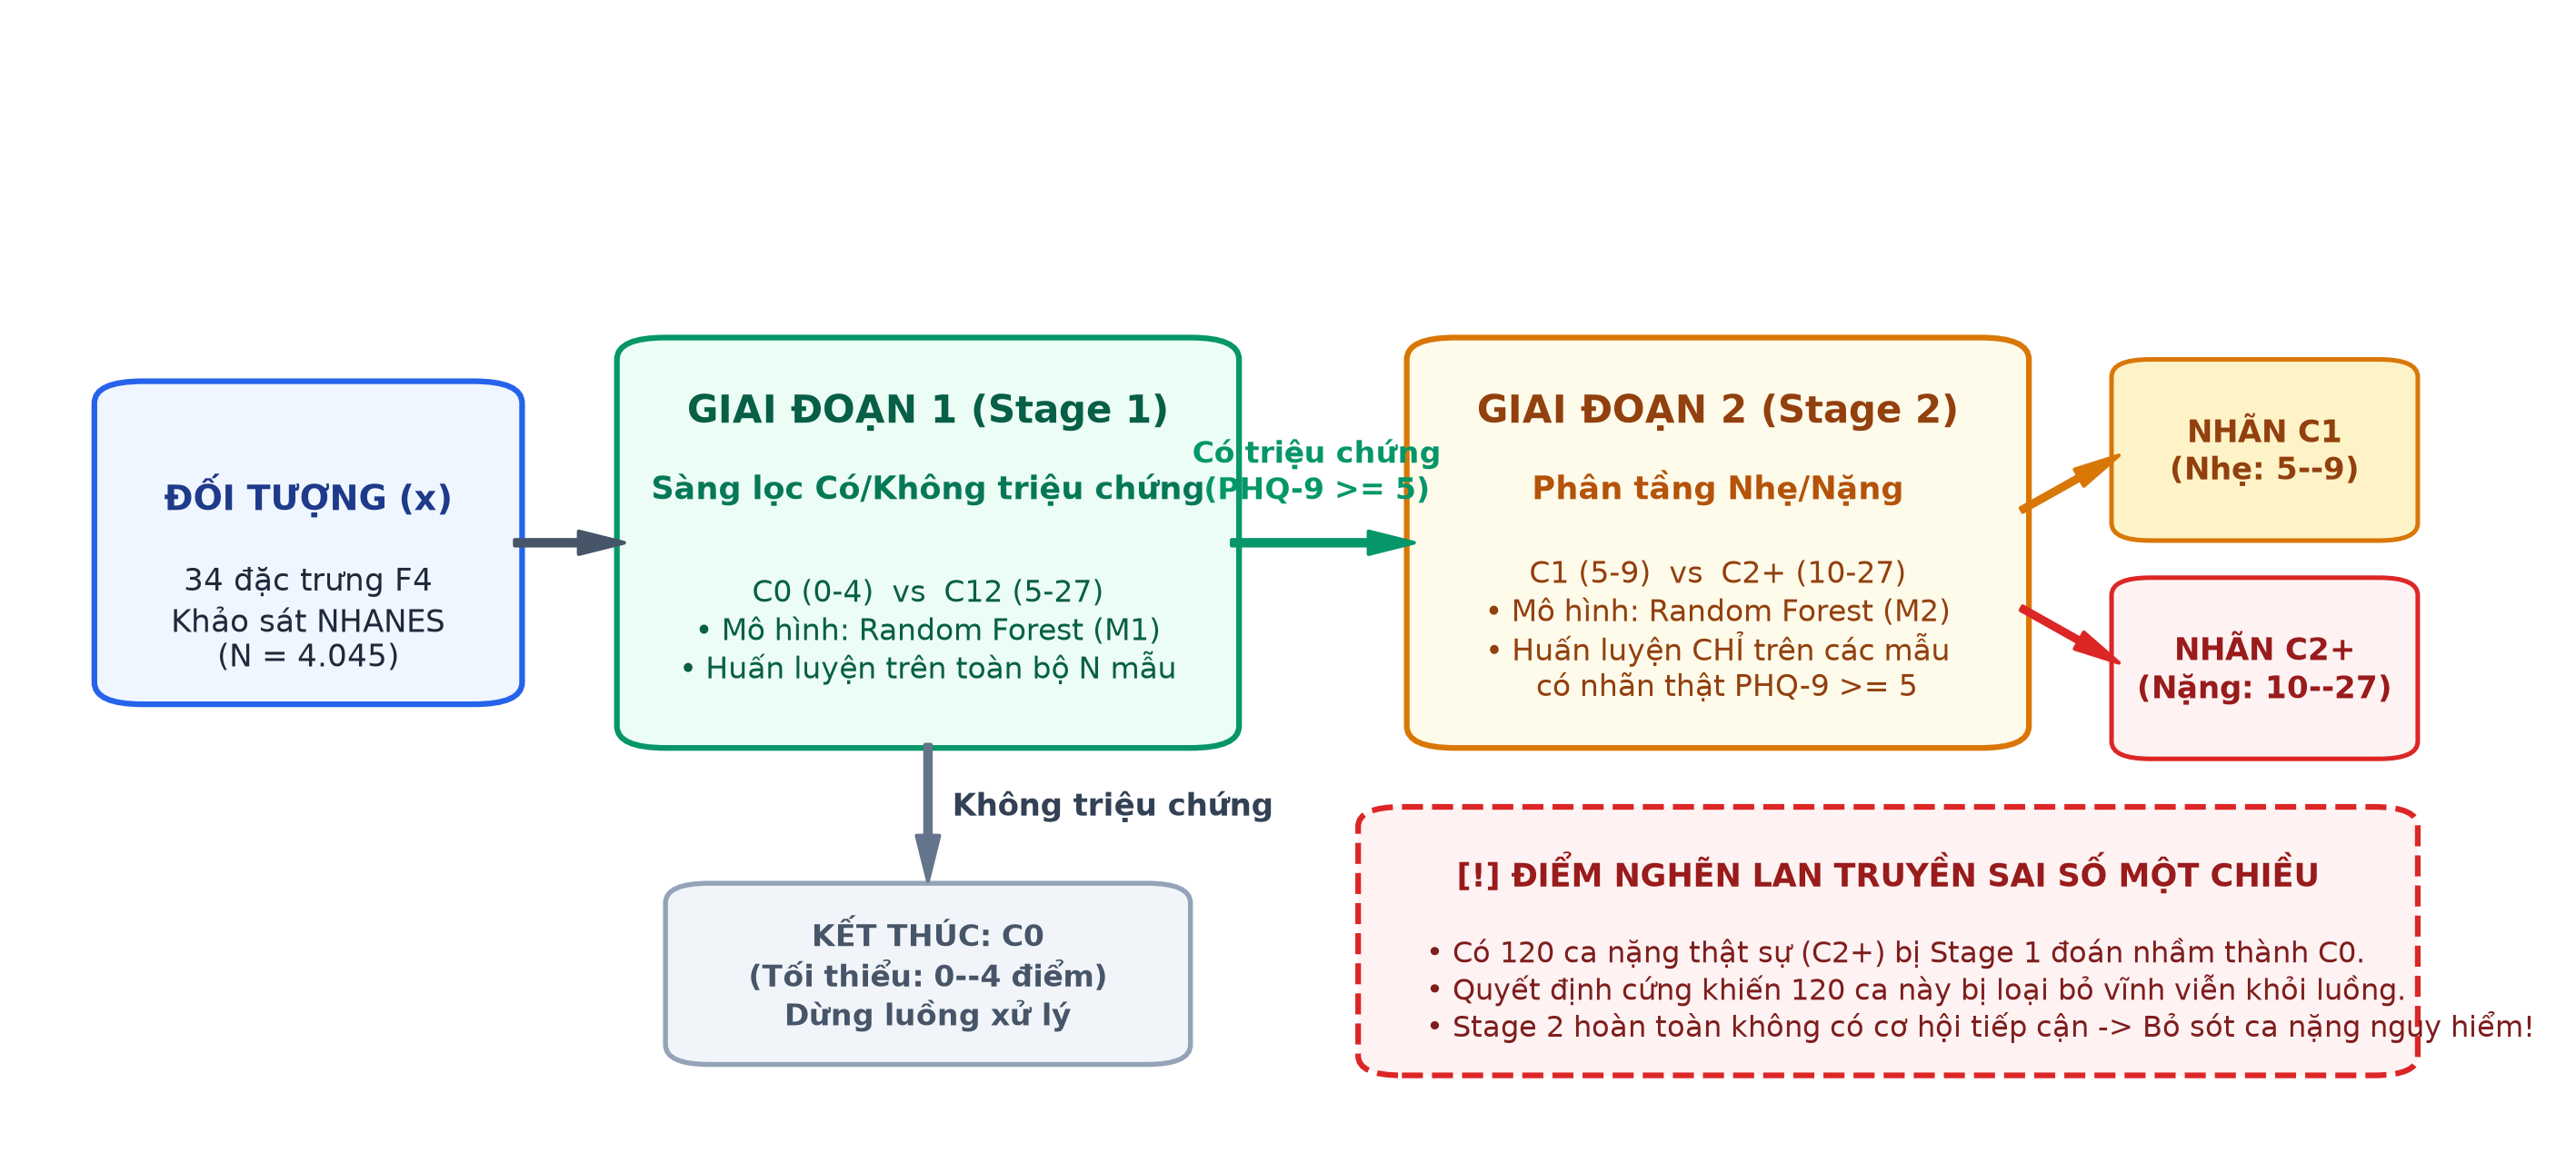
\includegraphics[width=\textwidth]{figures/fig3_4_hard_hierarchical.png}
\label{fig:hard-hierarchical}
\end{figure}
\FloatBarrier

\textbf{Điểm cốt lõi về tập dữ liệu huấn luyện của Random Forest trong hai giai đoạn:}
\begin{itemize}
    \item \textbf{Mô hình Stage 1 ($M_1$):} Thuật toán Random Forest được huấn luyện trên \textbf{TOÀN BỘ tập dữ liệu phát triển $N = 4.045$ đối tượng} (gồm $3.016$ ca $C_0$ và $1.029$ ca $C_{12}$).
    \item \textbf{Mô hình Stage 2 ($M_2$):} Thuật toán Random Forest được huấn luyện \textbf{RIÊNG BIỆT CHỈ TRÊN CÁC MẪU CÓ NHÃN THẬT $\text{PHQ-9} \ge 5$} ($N = 1.029$ đối tượng, gồm $638$ ca $C_1$ và $391$ ca $C_2^+$). Việc giới hạn tập huấn luyện này bảo đảm mô hình $M_2$ tập trung toàn bộ năng lực học máy vào việc phân biệt ranh giới giữa ca nhẹ và ca nặng, không bị chi phối bởi lớp đa số $C_0$.
\end{itemize}

\noindent\textbf{Nhấn mạnh phương pháp luận về bản chất độc lập của các mô hình Random Forest:} Cần khẳng định dứt khoát rằng mô hình Random Forest trong bài toán 5 lớp phẳng $T_5$ (huấn luyện trên 5 lớp đồng thời, $N=4.045$), mô hình RF Stage 1 trong $T_3$ (huấn luyện nhị phân $C_0$ vs $C_{12}$, $N=4.045$) và mô hình RF Stage 2 trong $T_3$ (huấn luyện nhị phân $C_1$ vs $C_2^+$, chỉ trên $N=1.029$ ca có triệu chứng thực tế) là \textbf{những mô hình hoàn toàn khác nhau, giải quyết các mục tiêu chẩn đoán khác nhau và được huấn luyện trên các không gian dữ liệu khác nhau}. Đồng thời, bài toán $T_3$ là một bài toán phân loại độc lập với không gian nhãn được tái cấu trúc, không phải là kết quả cải thiện trực tiếp trên cùng không gian 5 lớp.

Bốn cấu hình thực nghiệm phân cấp cứng được khảo sát:
\begin{itemize}
    \item $E_1$: Cấu hình thuần Rừng ngẫu nhiên (RF--RF) với siêu tham số mặc định.
    \item $E_2$: Cấu hình RF--RF tinh chỉnh siêu tham số và ngưỡng cắt độc lập trên từng giai đoạn.
    \item $E_{3a}$: Cấu hình lai ghép RF--LR (Stage 1 dùng RF, Stage 2 dùng Hồi quy Logistic) nhằm kiểm tra xem liệu một mô hình tuyến tính trơn mượt có giảm thiểu quá khớp tốt hơn RF trong không gian bị co hẹp $N = 1.029$.
    \item $E_{3b}$: Cấu hình lai ghép RF--XGBoost (Stage 1 dùng RF, Stage 2 dùng XGBoost) nhằm khảo sát khả năng tăng cường độ dốc trên các ca bệnh có triệu chứng.
\end{itemize}

\textbf{Điểm nghẽn lan truyền sai số (Error Propagation):} Do quyết định ở Giai đoạn 1 là quyết định cứng, bất kỳ đối tượng nào thuộc nhóm nặng $C_2^+$ bị $M_1$ gán nhầm thành $C_0$ sẽ bị loại bỏ hoàn toàn khỏi luồng xử lý và không bao giờ có cơ hội được $M_2$ xem xét lại. Đây là rủi ro lâm sàng nghiêm trọng của cơ chế định tuyến cứng, sẽ được định lượng cụ thể tại Chương \ref{ch:thuc-nghiem}.

\subsection{Kiến trúc phân loại phân cấp định tuyến mềm và tối ưu chi phí Bayes ($E_4 \to E_6$)}
\label{subsec:soft-cost-hierarchical}

Để khắc phục hiện tượng nghẽn sai số một chiều, kiến trúc phân cấp mềm (Hình \ref{fig:soft-cost-architecture}) chuyển toàn bộ quá trình ra quyết định sang miền xác suất liên tục.

\begin{figure}[htbp]{Kiến trúc phân loại phân cấp mềm kết hợp lý thuyết quyết định nhạy chi phí Bayes}
\centering
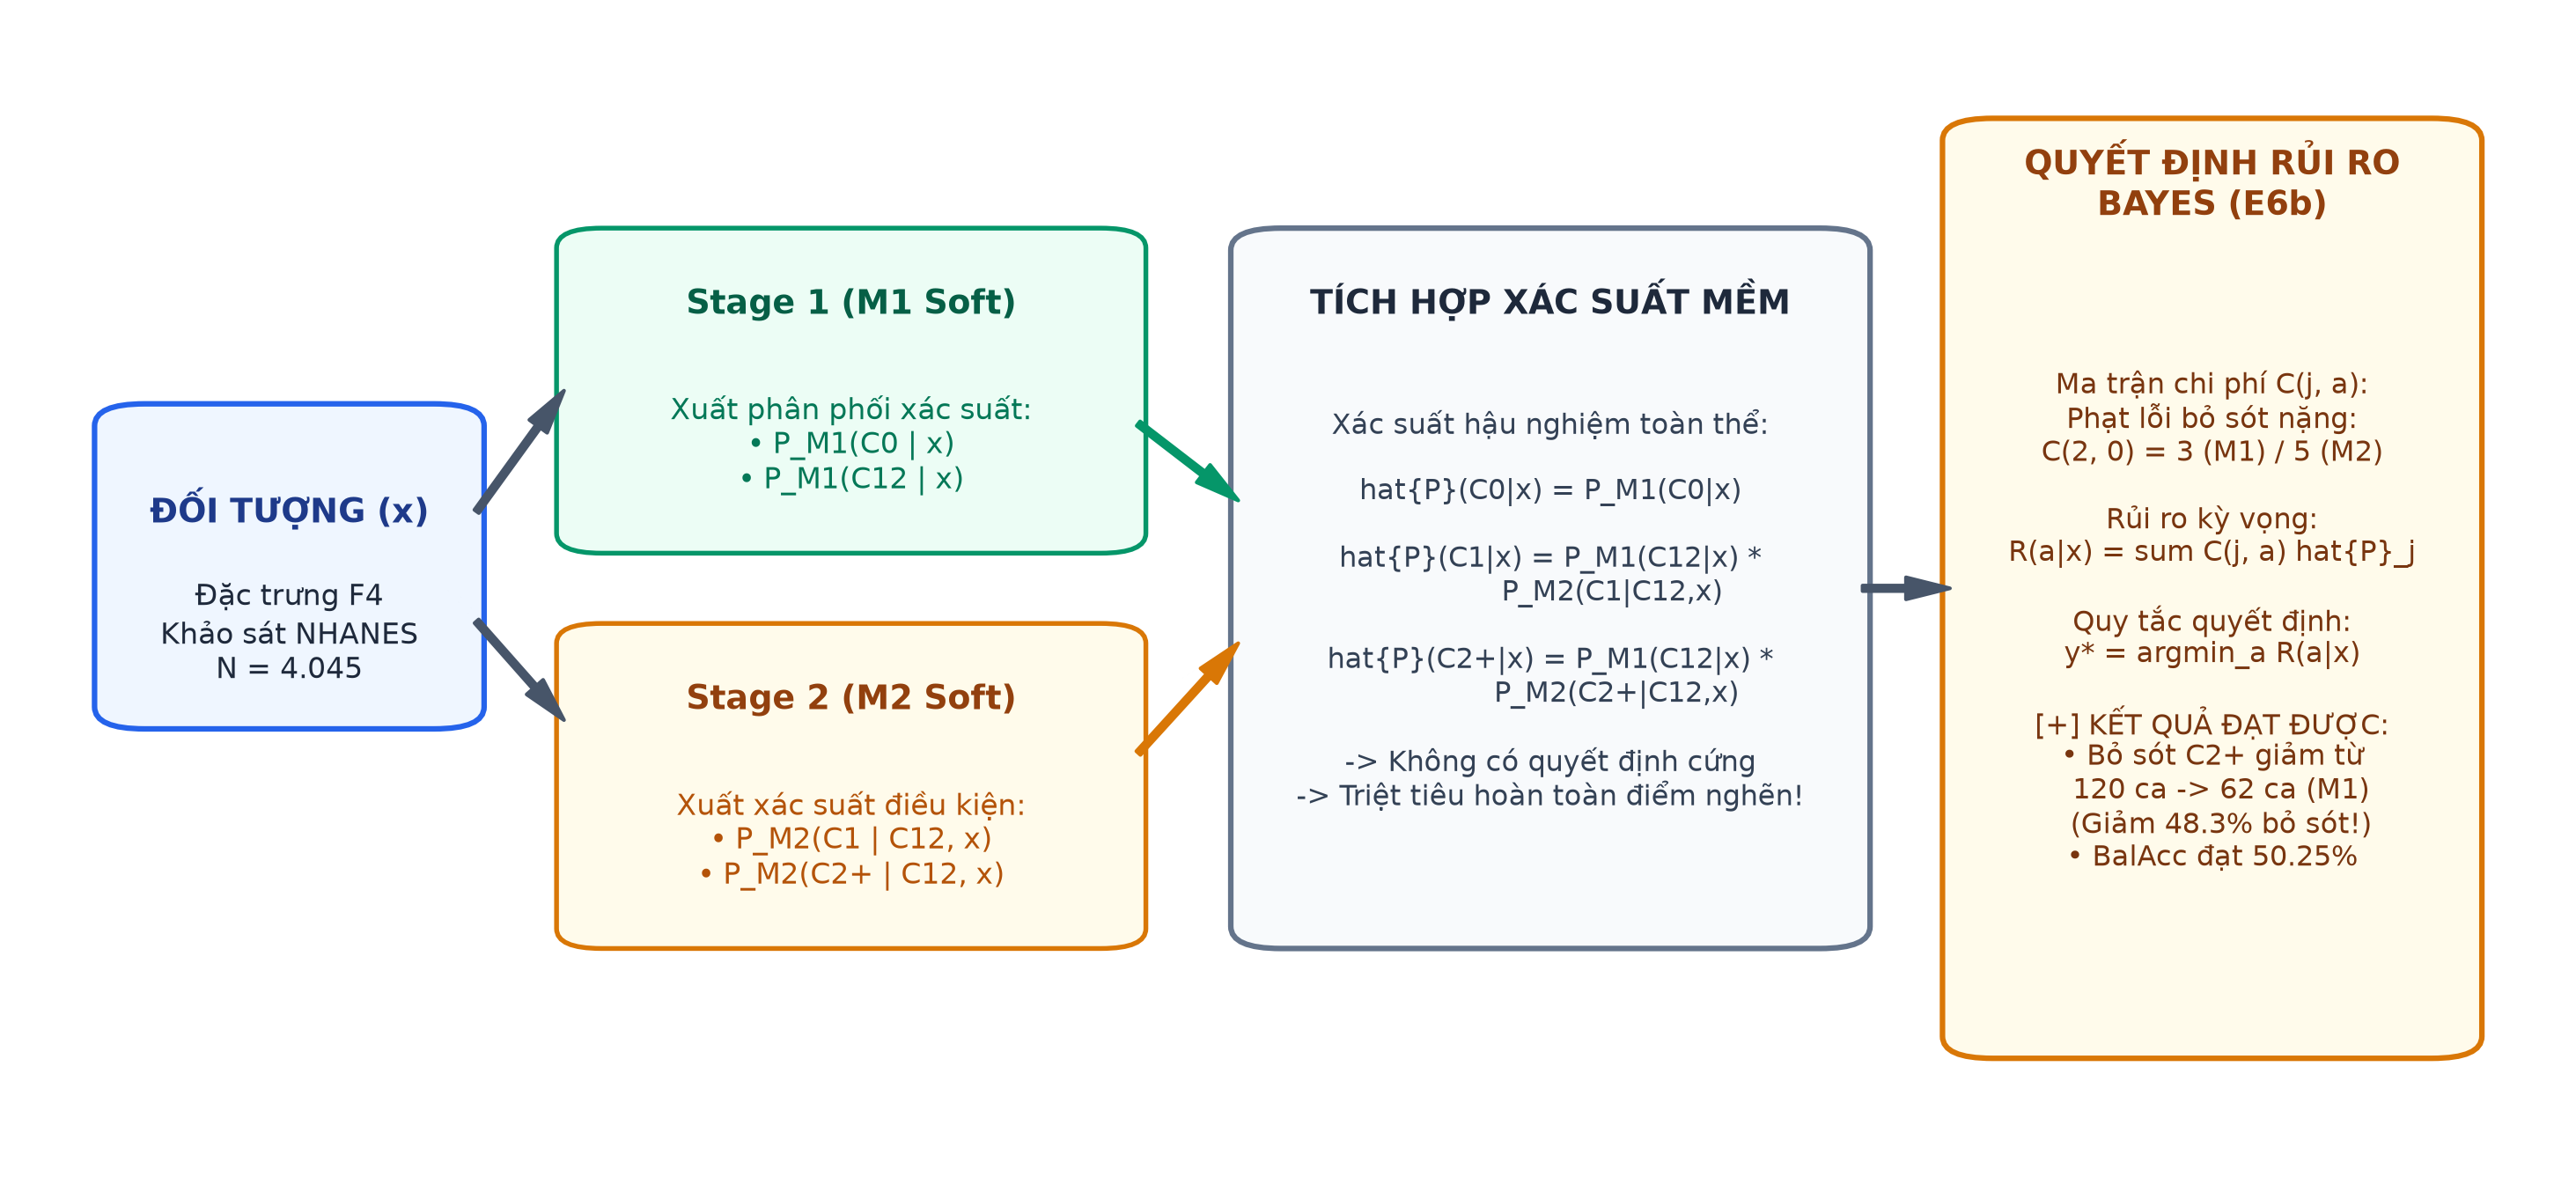
\includegraphics[width=\textwidth]{figures/fig3_5_soft_cost_sensitive.png}
\label{fig:soft-cost-architecture}
\end{figure}
\FloatBarrier

Phân phối xác suất hậu nghiệm đầy đủ $\hat{\mathbf{p}} = [\hat{P}(C_0), \hat{P}(C_1), \hat{P}(C_2^+)]^T$ được tổng hợp thông qua công thức xác suất toàn phần:
\begin{align}
    \hat{P}(C_0 \mid \mathbf{x}) &= P_{M_1}(C_0 \mid \mathbf{x}) \\
    \hat{P}(C_1 \mid \mathbf{x}) &= P_{M_1}(C_{12} \mid \mathbf{x}) \cdot P_{M_2}(C_1 \mid C_{12}, \mathbf{x}) \\
    \hat{P}(C_2^+ \mid \mathbf{x}) &= P_{M_1}(C_{12} \mid \mathbf{x}) \cdot P_{M_2}(C_2^+ \mid C_{12}, \mathbf{x})
\end{align}

Từ phân phối xác suất hậu nghiệm mềm, hai cơ chế ra quyết định được áp dụng:
\begin{enumerate}
    \item \textbf{Cơ chế Argmax không trọng số ($E_4, E_5$):} Chọn nhãn có xác suất cực đại $\hat{y} = \arg\max_k \hat{P}(C_k \mid \mathbf{x})$. Cấu hình $E_4$ sử dụng RF--RF; $E_5$ sử dụng RF--LR.
    \item \textbf{Cơ chế tối thiểu hóa rủi ro Bayes ($E_{6a}, E_{6b}$):} Đưa ma trận chi phí bất đối xứng $\mathbf{C} \in \mathbb{R}^{3 \times 3}$ vào hàm quyết định:
    \begin{equation}
        \hat{y}^* = \arg\min_{a \in \{0, 1, 2\}} \sum_{j=0}^2 \mathbf{C}(j, a) \hat{P}(C_j \mid \mathbf{x})
    \end{equation}
    trong đó $\mathbf{C}(j, a)$ là chi phí khi nhãn thực tế là $C_j$ nhưng mô hình dự đoán là $C_a$. Nghiên cứu khảo sát 4 ma trận chi phí từ $M_0$ (chi phí đồng nhất) đến $M_3$ (phạt nặng nhất sai số bỏ sót ca nặng $\mathbf{C}(2, 0) = 8.0$). Ma trận được sử dụng chính trong báo cáo là $M_1$ ($\mathbf{C}(2, 0) = 3.0$). Chi tiết ma trận chi phí được trình bày tại Phụ lục \ref{app:cost-matrices}.
\end{enumerate}

\subsection{Mô hình phân loại thứ bậc ($E_7$)}
\label{subsec:e7-ordinal}

Do các mức độ triệu chứng PHQ-9 có tính chất thứ bậc tự nhiên ($C_0 < C_1 < C_2^+$), họ mô hình $E_7$ khai thác trực tiếp mối quan hệ trật tự này (Hình \ref{fig:ordinal-architecture}):
\begin{itemize}
    \item $E_{7a}$ (Balanced Ordinal Logistic Regression -- Balanced OLR): Mô hình hồi quy logistic thứ bậc với giả định tỷ lệ chênh tỉ lệ thuận (proportional odds) và hàm phạt cân bằng tần số lớp.
    \item $E_{7b}$ (Cumulative Binary Classification -- CumBin RF): Huấn luyện 2 bộ phân loại nhị phân tích lũy độc lập $P(Y \ge 1)$ và $P(Y \ge 2)$ bằng Random Forest, kết hợp thuật toán hiệu chỉnh nhằm khắc phục hiện tượng vi phạm tính đơn điệu xác suất.
\end{itemize}

\begin{figure}[htbp]{Kiến trúc các phương pháp phân loại thứ bậc trong DepSev-ML ($E_{7a}$ và $E_{7b}$)}
\centering
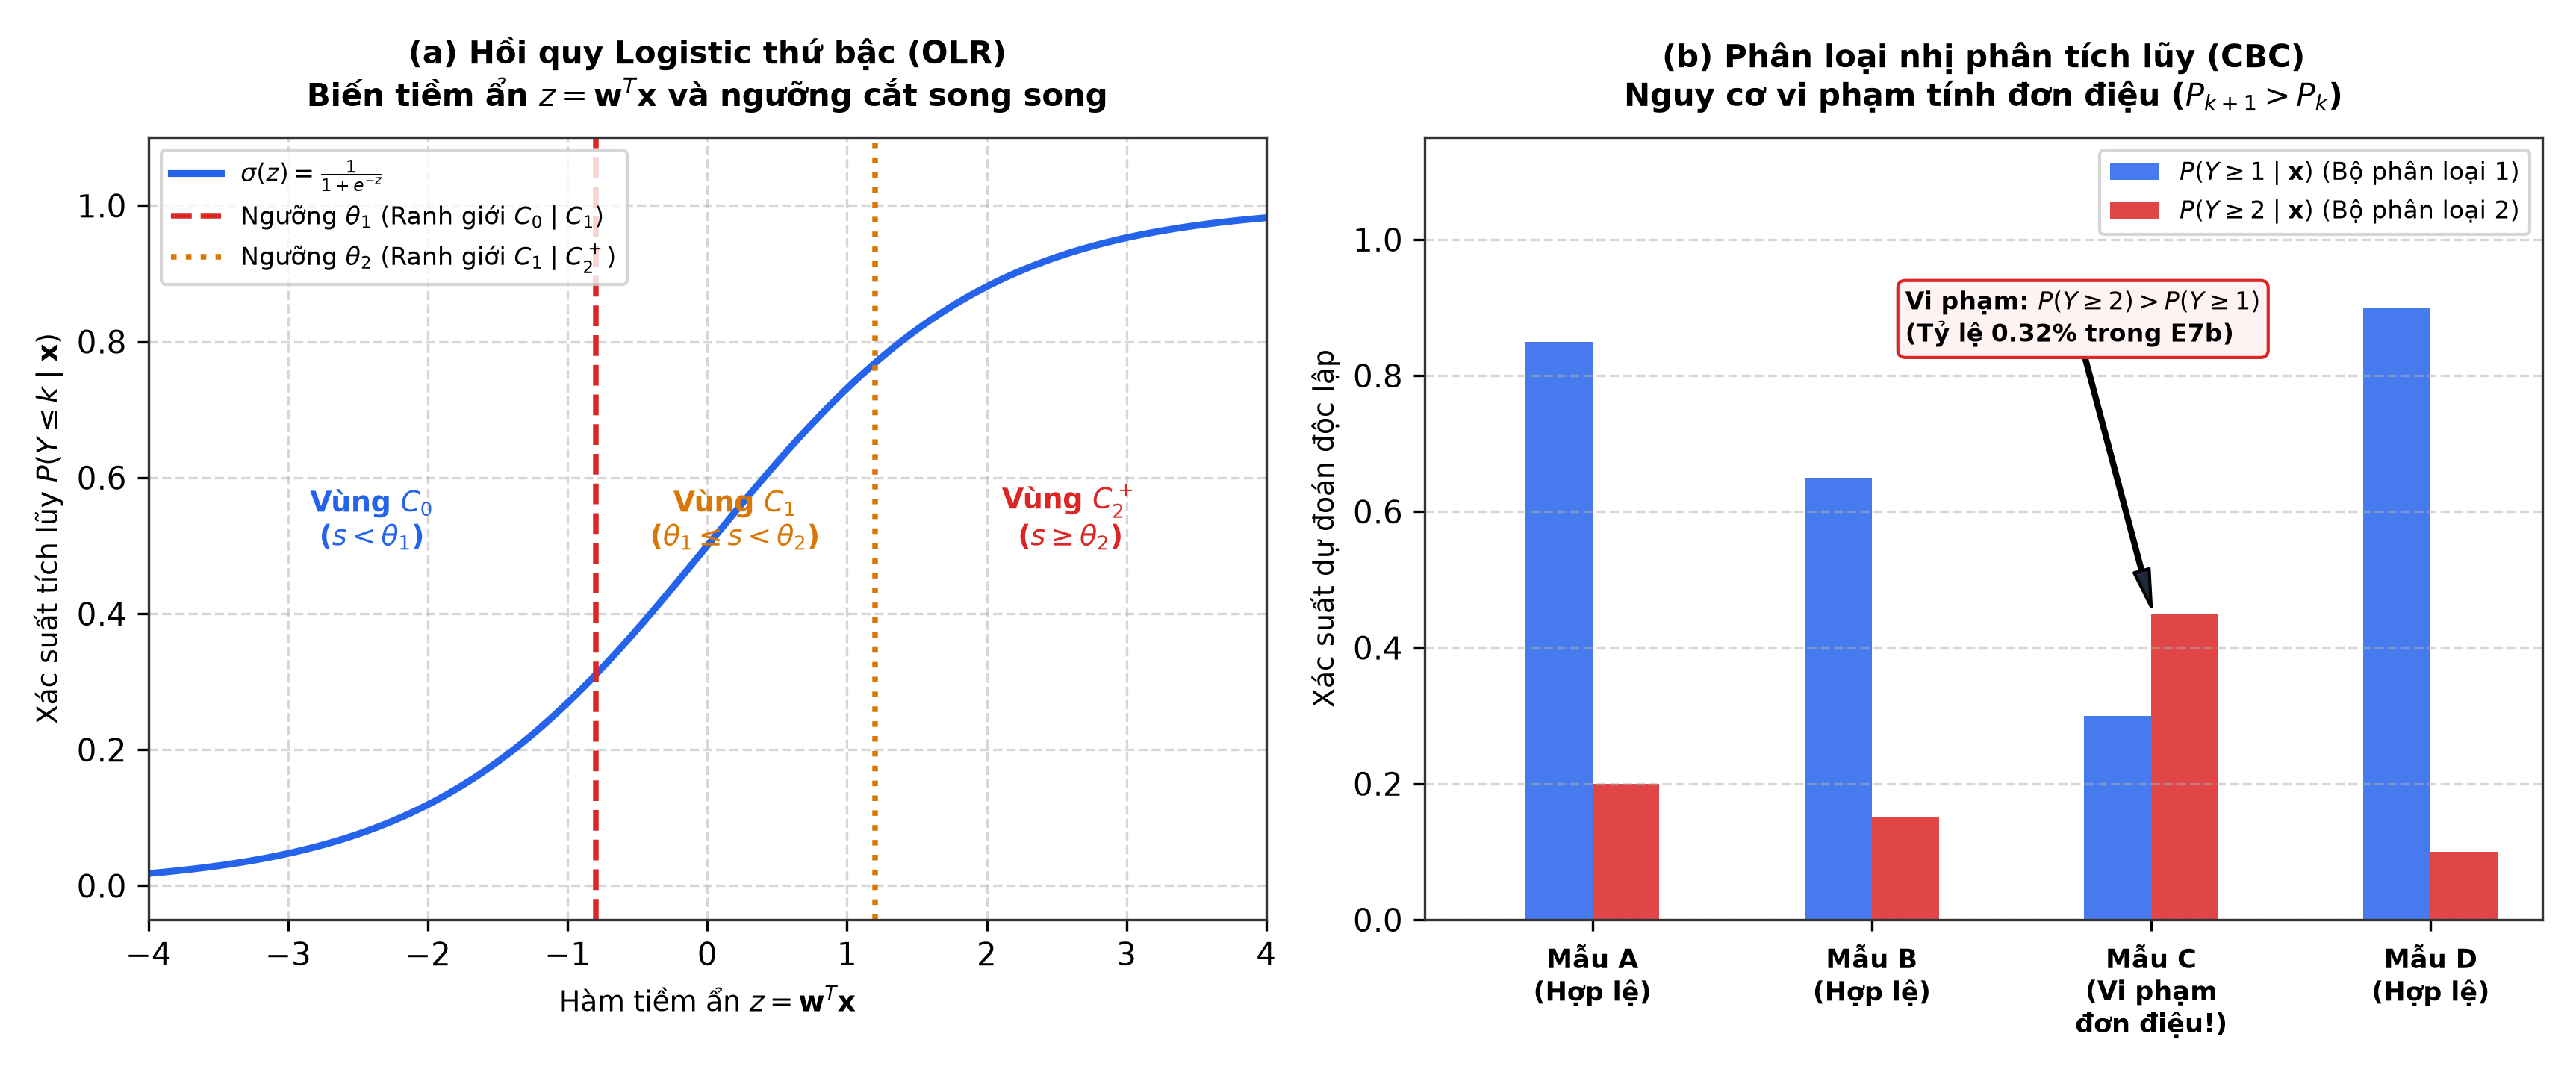
\includegraphics[width=0.9\textwidth]{figures/fig3_6_ordinal_classification.png}
\label{fig:ordinal-architecture}
\end{figure}
\FloatBarrier
\label{subsec:ordinal-models}

Nhóm thực nghiệm $E_7$ khai thác trật tự tự nhiên $C_0 < C_1 < C_2^+$ thông qua hai phương pháp (Hình \ref{fig:ordinal-classification}):

\begin{figure}[htbp]{Nguyên lý mô hình hóa thứ bậc: (a) Hồi quy Logistic thứ bậc và (b) Phân loại nhị phân tích lũy}
\centering
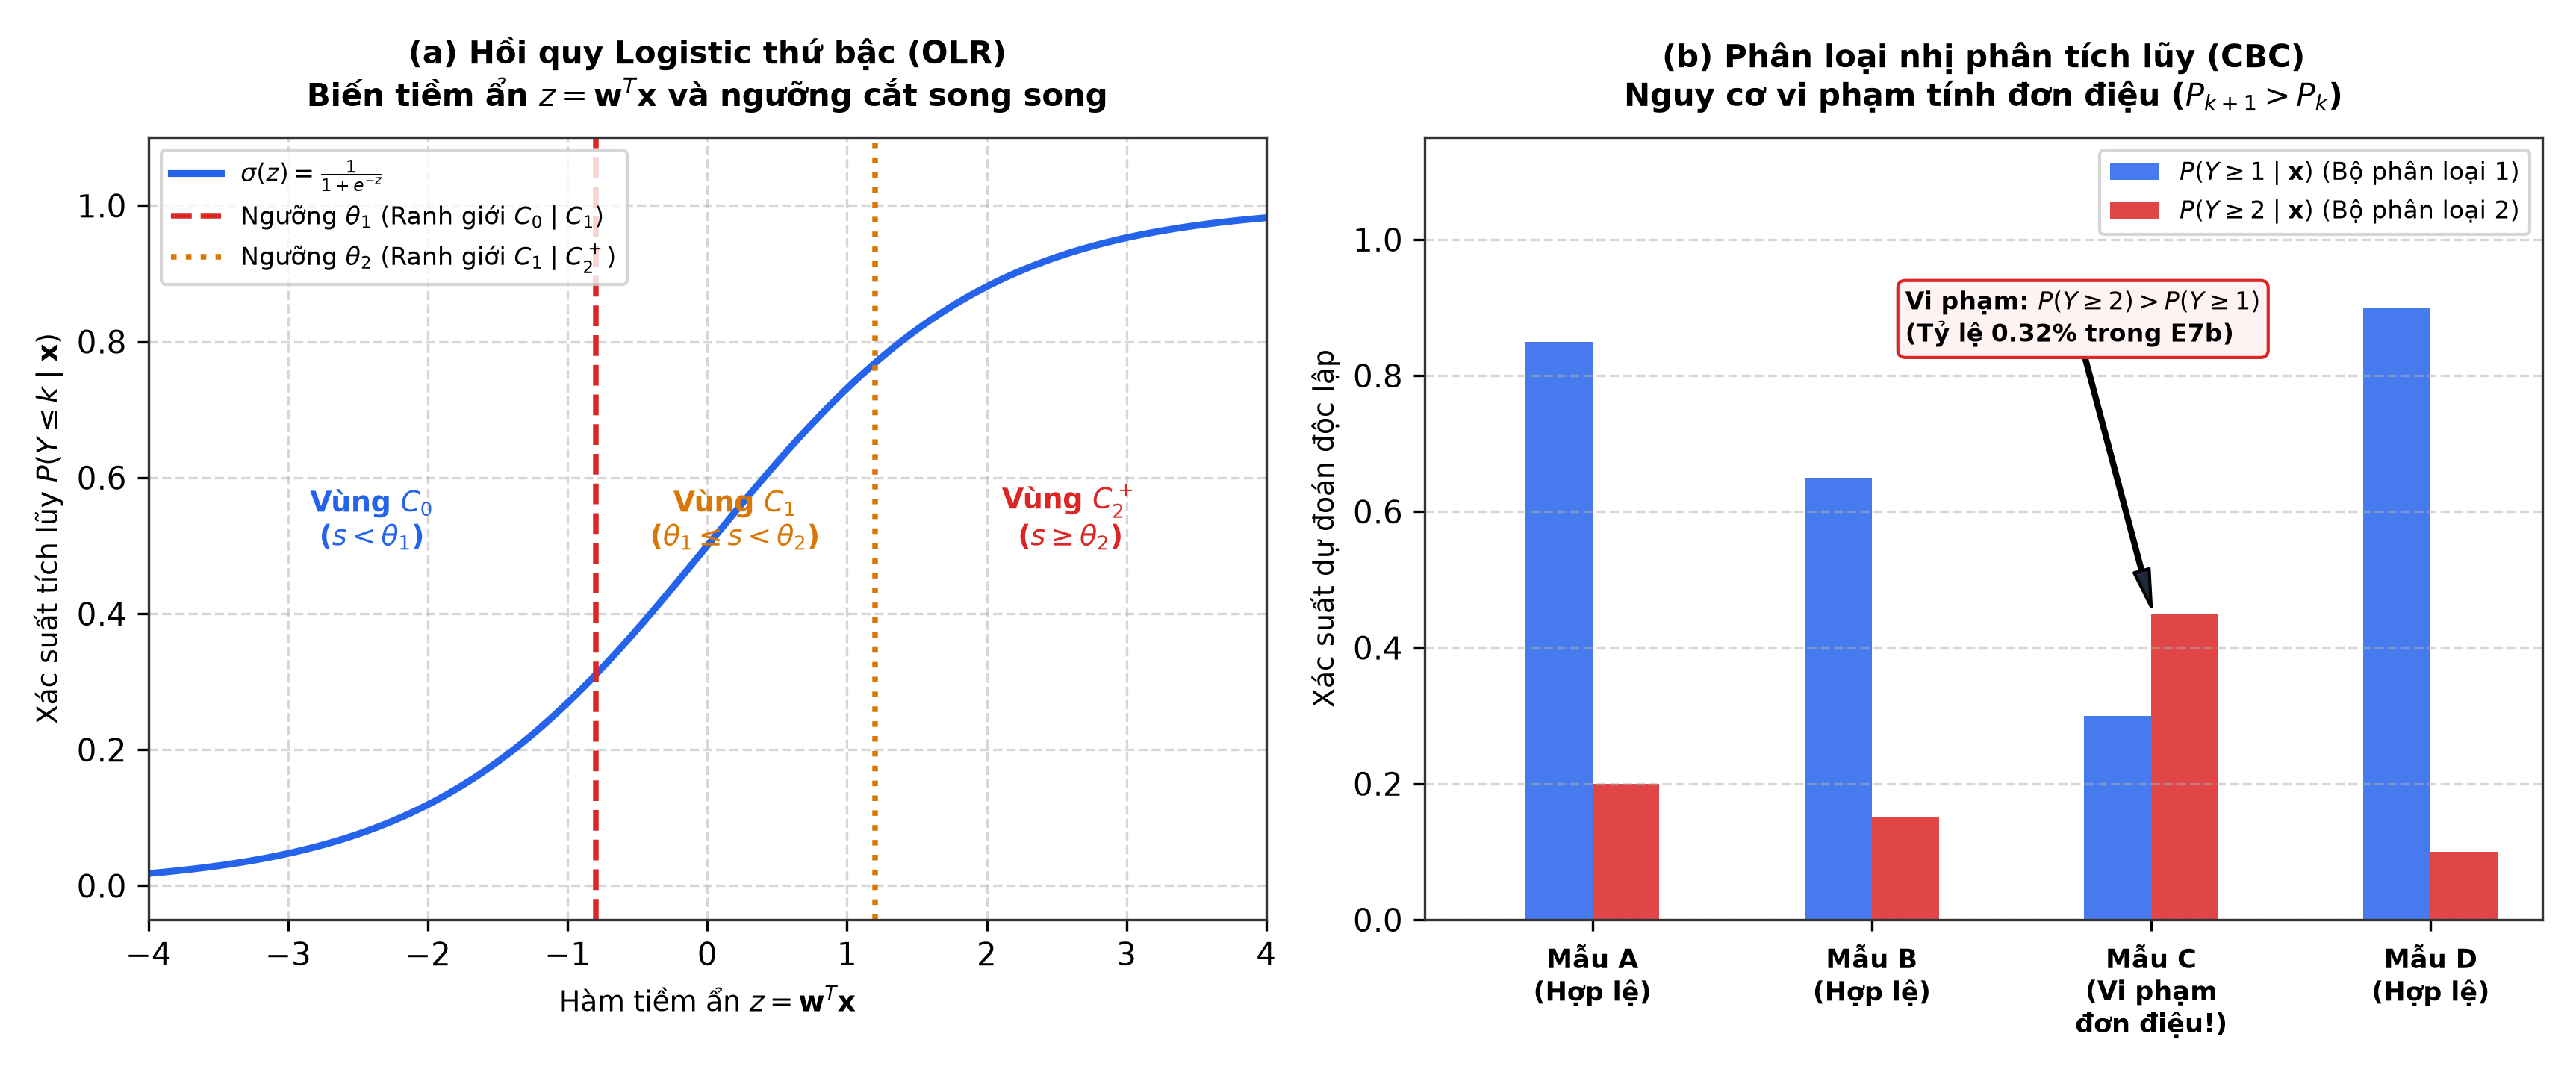
\includegraphics[width=\textwidth]{figures/fig3_6_ordinal_classification.png}
\label{fig:ordinal-classification}
\end{figure}
\FloatBarrier

\begin{enumerate}
    \item \textbf{Hồi quy Logistic thứ bậc ($E_{7a}$ -- OLR):} 
    Mô hình giả định biến tiềm ẩn $z = \mathbf{w}^T \mathbf{x}$ cùng hai ngưỡng cắt $\theta_1 < \theta_2$. Xác suất tích lũy được mô hình hóa qua hàm phân phối Logistic:
    \begin{equation}
        P(Y \le k \mid \mathbf{x}) = \sigma(\theta_{k+1} - \mathbf{w}^T \mathbf{x}) = \frac{1}{1 + e^{-(\theta_{k+1} - \mathbf{w}^T \mathbf{x})}}
    \end{equation}
    Nghiên cứu khảo sát hai phiên bản: $E_{7a}$ Unweighted và $E_{7a}$ Balanced (gán trọng số nghịch đảo tần số lớp).
    \item \textbf{Phân loại nhị phân tích lũy ($E_{7b}$ -- Cumulative Binary Classification):} 
    Huấn luyện hai bộ phân loại nhị phân độc lập $h_1(\mathbf{x})$ cho bài toán $Y \ge 1$ và $h_2(\mathbf{x})$ cho bài toán $Y \ge 2$. Xác suất từng lớp được suy luận bằng hiệu số tích lũy: $P(Y=0) = 1 - P(Y \ge 1)$, $P(Y=1) = P(Y \ge 1) - P(Y \ge 2)$, $P(Y=2) = P(Y \ge 2)$. Nếu xảy ra vi phạm đơn điệu $P(Y \ge 2) > P(Y \ge 1)$, giải thuật hiệu chỉnh ngưỡng cắt (isotonic clipping) được kích hoạt.
\end{enumerate}

\section{Thiết kế giao thức kiểm thử thực nghiệm}
\label{sec:giao-thuc-kiem-thu}

Để bảo đảm độ tin cậy khoa học cao nhất, DepSev-ML áp dụng hai tầng giao thức kiểm định độc lập được minh họa trong Hình \ref{fig:evaluation-protocol}.

\begin{figure}[htbp]{Hai tầng giao thức kiểm thử: Nested 5-Fold Stratified CV và Temporal Validation}
\centering
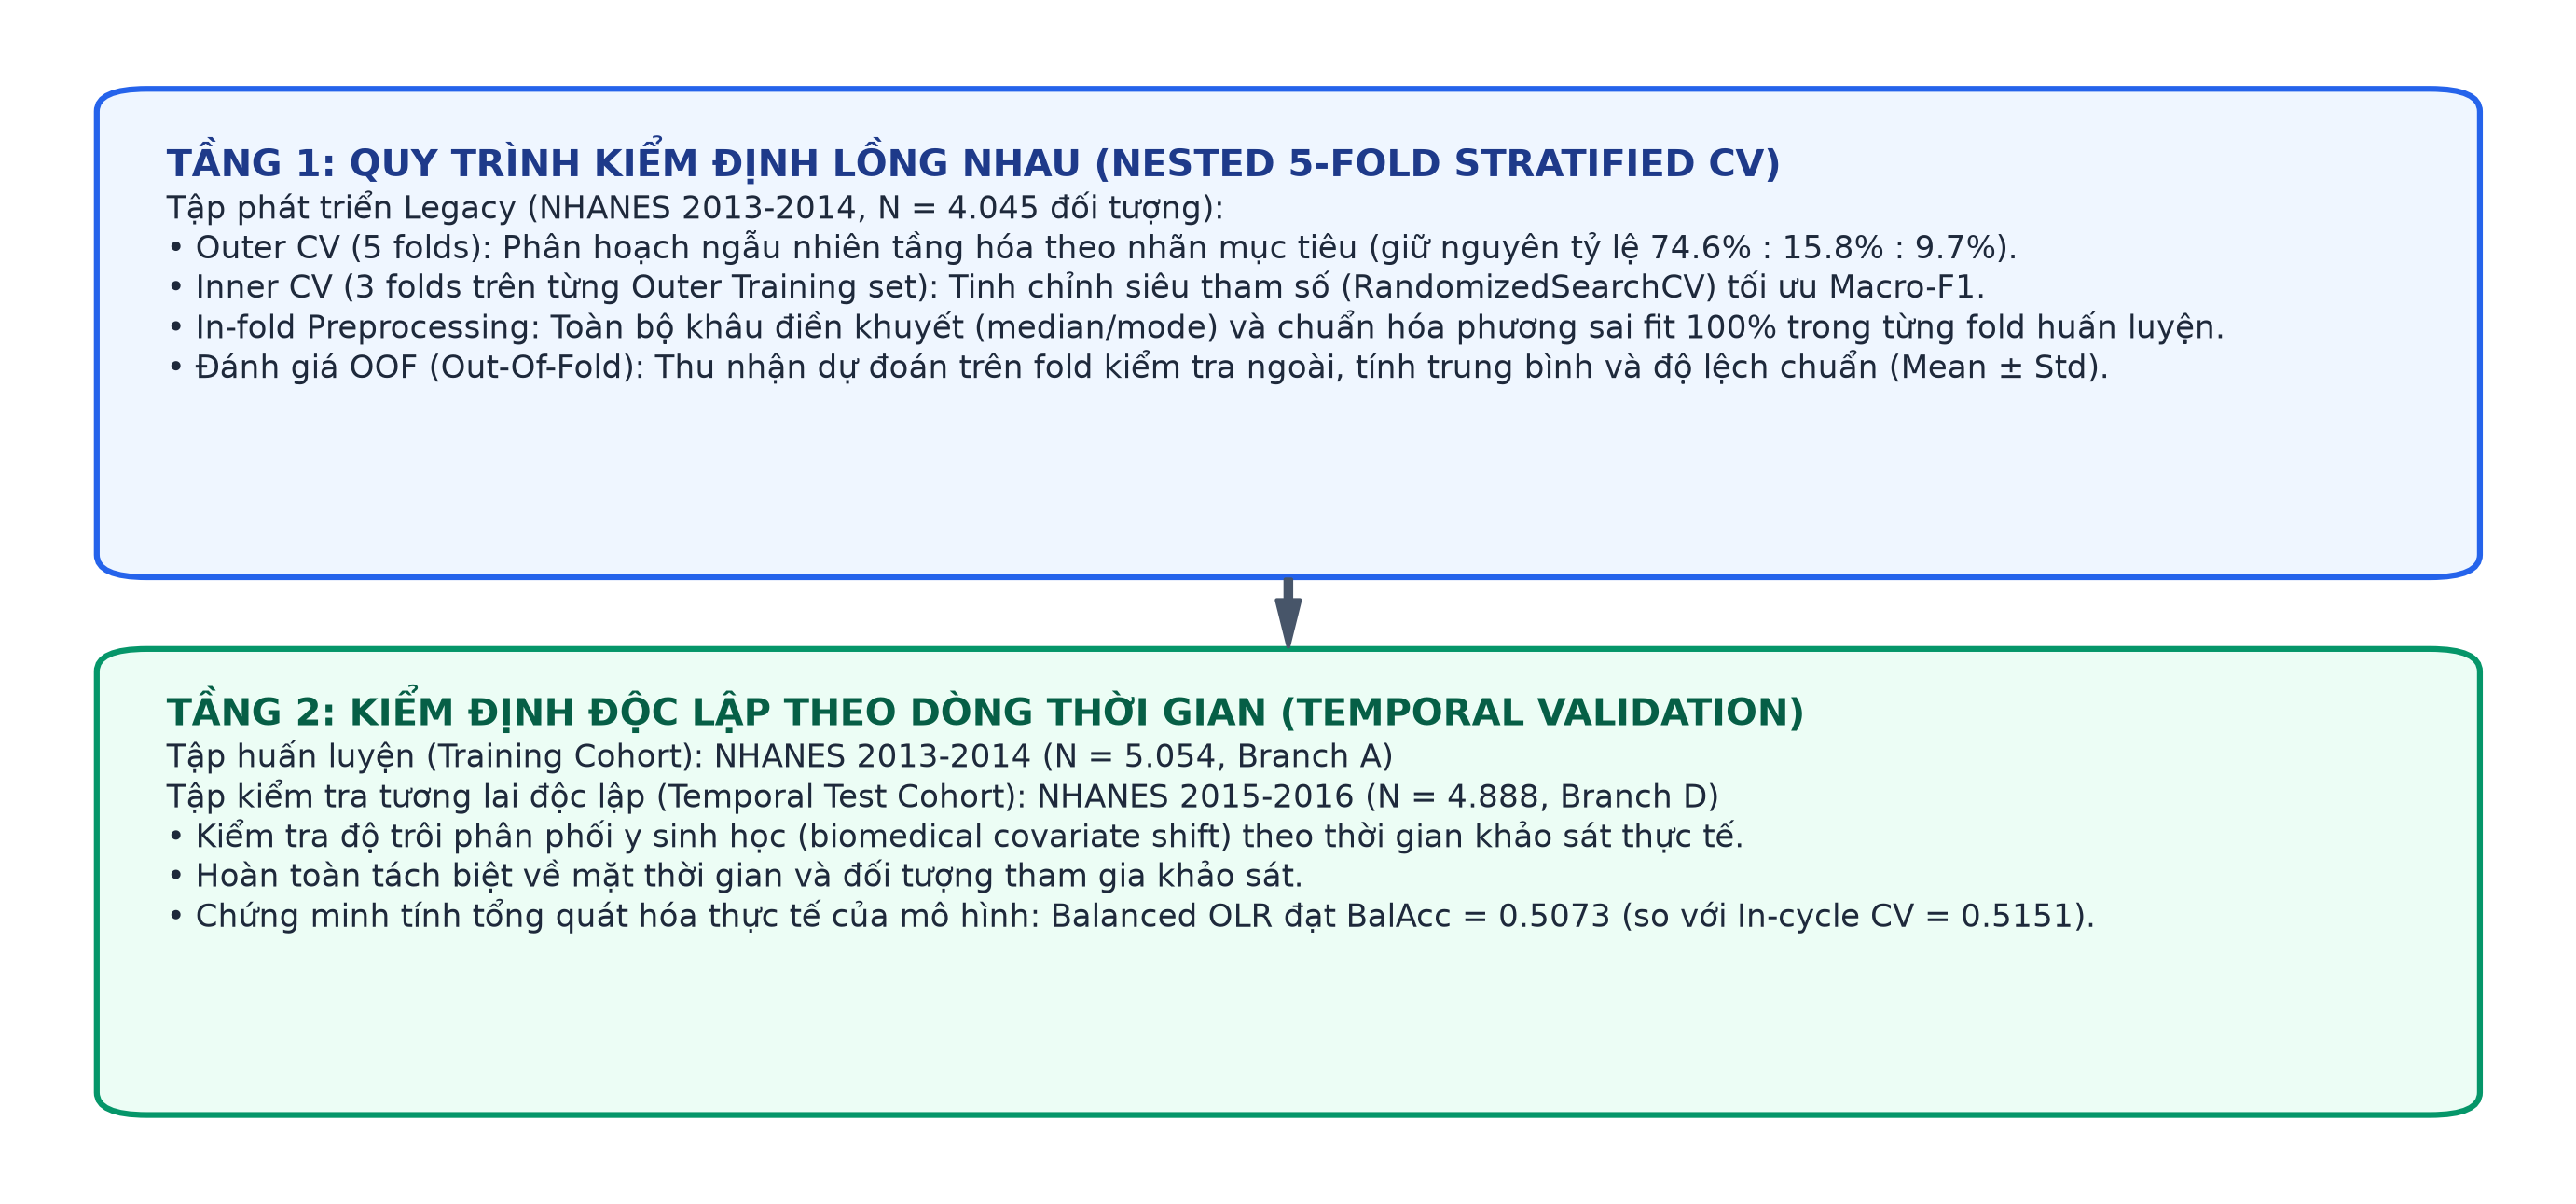
\includegraphics[width=\textwidth]{figures/fig3_7_evaluation_protocol.png}
\label{fig:evaluation-protocol}
\end{figure}
\FloatBarrier

\subsection{Quy trình kiểm định chéo lồng nhau (Nested 5-Fold Stratified CV)}
\label{subsec:nested-cv-protocol}

Trên tập dữ liệu phát triển Legacy ($N = 4.045$), quy trình kiểm định chéo lồng nhau được thực thi như sau:
\begin{itemize}
    \item \textbf{Outer CV (5 folds):} Phân chia dữ liệu thành 5 phần ngẫu nhiên có bảo toàn tỷ lệ lớp (Stratified Split). Tại mỗi vòng lặp, 4 fold được dùng để huấn luyện và 1 fold dùng để đánh giá ngoài mẫu (Out-Of-Fold -- OOF).
    \item \textbf{Inner CV (3 folds trên từng Outer Training set):} Thực hiện \texttt{RandomizedSearchCV} với 12 cấu hình siêu tham số ngẫu nhiên trên độ đo Macro-F1 nhằm tìm kiếm siêu tham số tối ưu mà không nhìn thấy dữ liệu kiểm tra của Outer fold.
    \item Kết quả báo cáo là giá trị trung bình kèm độ lệch chuẩn ($\text{Mean} \pm \text{Std}$) trên 5 outer folds.
\end{itemize}

\subsection{Giao thức kiểm định độc lập theo dòng thời gian (Temporal Validation)}
\label{subsec:temporal-protocol}

Nhằm kiểm tra tính bền vững của các mô hình trước hiện tượng trôi phân phối y sinh theo thời gian (covariate shift), nghiên cứu thiết lập giao thức kiểm định ngoại suy (Branch D): Tập huấn luyện gồm dữ liệu gộp hai chu kỳ quá khứ NHANES 2011--2012 và 2013--2014 ($N = 9.693$); Tập kiểm tra độc lập gồm toàn bộ chu kỳ tương lai NHANES 2015--2016 ($N = 4.888$), áp dụng trên không gian 31 đặc trưng sinh lý hài hòa hóa ($F_{4\_\text{common31}}$). Hai tập dữ liệu hoàn toàn tách biệt về mặt thời gian khảo sát và không có bất kỳ đối tượng nào trùng lặp.

\section{Hệ thống độ đo đánh giá đa chiều}
\label{sec:he-thong-do-do}

Nghiên cứu thiết lập bộ chỉ số đánh giá đa chiều:
\begin{enumerate}
    \item \textbf{Macro-F1:} Trung bình cộng F1-score của toàn bộ các lớp, phản ánh năng lực phân biệt đồng đều không phụ thuộc quy mô lớp.
    \item \textbf{Balanced Accuracy (BalAcc):} Trung bình cộng của Recall từng lớp $\text{BalAcc} = \frac{1}{K}\sum_k \text{Recall}_k$.
    \item \textbf{Class MAE (Sai số tuyệt đối theo lớp):} Đo lường khoảng cách trung bình giữa mức độ dự đoán và mức độ thực tế: $\text{Class MAE} = \frac{1}{N} \sum_{i=1}^N |y_i - \hat{y}_i|$.
    \item \textbf{Quadratic Weighted Kappa (QWK):} Đo lường mức độ đồng thuận thứ bậc có phạt nặng các lỗi nhảy bậc xa \cite{cohen1968weighted}.
    \item \textbf{Chỉ số an toàn lâm sàng (Clinical Safety Metrics):} Số lượng ca nặng bị bỏ sót thành bình thường ($C_2^+ \to C_0$) và số ca báo động nhầm ($C_0 \to C_2^+$).
\end{enumerate}

\section{Tóm tắt chương}
\label{sec:tom-tat-chuong-3}

Chương 3 đã xây dựng toàn diện phương pháp luận cho đề tài DepSev-ML: từ kiến trúc hệ thống 7 module, nguồn dữ liệu và giao thức tiền xử lý in-fold bảo toàn nguyên tắc Zero Data Leakage, 4 không gian đặc trưng lũy tiến ($F_1 \to F_4$), 8 thiết kế mô hình thực nghiệm đa trường phái ($E_0 \to E_7$), đến hai tầng giao thức kiểm thử khắt khe. Toàn bộ các kết quả thực nghiệm thu được từ phương pháp này sẽ được phân tích chi tiết trong Chương \ref{ch:thuc-nghiem}.

